\section{Liên hệ giữa đạo hàm và tính chất của hàm}
\label{sec:derivative-properties}

\subsection{Tính tăng, giảm, và cực trị}
\label{subsec:monotonicity-extrema}

Một trong những ứng dụng cơ bản nhất của đạo hàm là xác định các khoảng mà hàm số tăng hoặc giảm. Các khái niệm này được định nghĩa một cách chặt chẽ như sau:

\begin{definition}
Cho hàm số $f$ xác định trên một khoảng $I$.
\begin{itemize}
    \item $f$ được gọi là \textbf{tăng} trên $I$ nếu với mọi $x_1, x_2 \in I$ mà $x_1 < x_2$, ta có $f(x_1) \le f(x_2)$.
    \item $f$ được gọi là \textbf{tăng ngặt} trên $I$ nếu với mọi $x_1, x_2 \in I$ mà $x_1 < x_2$, ta có $f(x_1) < f(x_2)$.
    \item $f$ được gọi là \textbf{giảm} trên $I$ nếu với mọi $x_1, x_2 \in I$ mà $x_1 < x_2$, ta có $f(x_1) \ge f(x_2)$.
    \item $f$ được gọi là \textbf{giảm ngặt} trên $I$ nếu với mọi $x_1, x_2 \in I$ mà $x_1 < x_2$, ta có $f(x_1) > f(x_2)$.
\end{itemize}
Một hàm số được gọi chung là \textbf{đơn điệu} nếu nó là hàm tăng hoặc hàm giảm.
\end{definition}

Về mặt hình học, đồ thị của một hàm tăng sẽ đi lên (hoặc đi ngang) khi ta di chuyển từ trái sang phải. Ngược lại, đồ thị của một hàm giảm sẽ đi xuống (hoặc đi ngang). Dấu của đạo hàm cấp một là một công cụ hiệu quả để xác định các khoảng đơn điệu này.

\begin{theorem}[Tiêu chuẩn cho tính đơn điệu]
\label{thm:monotonicity-test}
Giả sử $f$ liên tục trên $[a, b]$ và khả vi trên $(a, b)$.
\begin{enumerate}[label=(\alph*)]
    \item Nếu $f'(x) > 0$ với mọi $x \in (a, b)$, thì $f$ tăng ngặt trên $[a, b]$.
    \item Nếu $f'(x) < 0$ với mọi $x \in (a, b)$, thì $f$ giảm ngặt trên $[a, b]$.
    \item Nếu $f'(x) = 0$ với mọi $x \in (a, b)$, thì $f$ là hàm hằng trên $[a, b]$.
\end{enumerate}
\end{theorem}

\begin{proof}
Đây là một ứng dụng trực tiếp của Định lý Giá trị Trung bình (\ref{thm:mean-value-theorem}).
Lấy hai điểm bất kỳ $x_1, x_2$ trong $[a,b]$ sao cho $x_1 < x_2$. Theo Định lý Giá trị Trung bình, tồn tại một số $c \in (x_1, x_2)$ sao cho:
$$ f(x_2) - f(x_1) = f'(c)(x_2 - x_1) $$
Vì $x_2 - x_1 > 0$, dấu của $f(x_2) - f(x_1)$ sẽ cùng dấu với $f'(c)$.
\begin{enumerate}[label=(\alph*)]
    \item Nếu $f'(x) > 0$ trên $(a,b)$, thì $f'(c) > 0$. Do đó $f(x_2) - f(x_1) > 0$, hay $f(x_2) > f(x_1)$. Vậy $f$ tăng ngặt.
    \item Nếu $f'(x) < 0$ trên $(a,b)$, thì $f'(c) < 0$. Do đó $f(x_2) - f(x_1) < 0$, hay $f(x_2) < f(x_1)$. Vậy $f$ giảm ngặt.
    \item Nếu $f'(x) = 0$ trên $(a,b)$, thì $f'(c) = 0$. Do đó $f(x_2) - f(x_1) = 0$, hay $f(x_2) = f(x_1)$. Vậy $f$ là hàm hằng.
\end{enumerate}
\end{proof}

Tiêu chuẩn trên dẫn đến một phương pháp hiệu quả để tìm các điểm cực trị địa phương, được gọi là \textbf{Tiêu chuẩn đạo hàm bậc nhất}.

\begin{theorem}[Tiêu chuẩn đạo hàm bậc nhất cho cực trị]
\label{thm:first-derivative-test}
Giả sử $c$ là một điểm tới hạn của hàm số $f$ và $f$ liên tục tại $c$.
\begin{enumerate}[label=(\alph*)]
    \item Nếu $f'(x)$ đổi dấu từ dương sang âm tại $c$ (tức là $f'(x)>0$ ở bên trái $c$ và $f'(x)<0$ ở bên phải $c$), thì $f$ có một \textbf{cực đại địa phương} tại $c$.
    \item Nếu $f'(x)$ đổi dấu từ âm sang dương tại $c$ (tức là $f'(x)<0$ ở bên trái $c$ và $f'(x)>0$ ở bên phải $c$), thì $f$ có một \textbf{cực tiểu địa phương} tại $c$.
    \item Nếu $f'(x)$ không đổi dấu tại $c$ (cùng dương hoặc cùng âm ở cả hai phía), thì $f$ không có cực trị địa phương tại $c$.
\end{enumerate}
\end{theorem}
\begin{proof}
(a) Nếu $f'(x) > 0$ ở bên trái $c$, thì theo Định lý \ref{thm:monotonicity-test}, $f$ tăng trên một khoảng $(a,c)$. Do đó $f(x) \le f(c)$ với mọi $x \in (a,c)$. Nếu $f'(x) < 0$ ở bên phải $c$, thì $f$ giảm trên một khoảng $(c,b)$. Do đó $f(x) \le f(c)$ với mọi $x \in (c,b)$. Vậy, $f(x) \le f(c)$ trên toàn bộ lân cận $(a,b)$, suy ra $f$ có cực đại địa phương tại $c$.
Phần (b) và (c) được chứng minh tương tự.
\end{proof}

Những hàm số có đạo hàm liên tục thường được gọi là các \textbf{hàm trơn}. Tên gọi này xuất phát từ ý nghĩa hình học: đồ thị của một hàm trơn là một đường cong mượt mà, không có ``góc nhọn'', và phương của tiếp tuyến thay đổi một cách liên tục. Đối với các hàm trơn, các điểm tới hạn chính là các điểm dừng, và dấu của đạo hàm $f'$ sẽ không đổi giữa hai điểm dừng liên tiếp. Điều này đơn giản hóa rất nhiều việc khảo sát hàm số.
\begin{importantbox}
\textbf{Quy trình khảo sát tính đơn điệu và tìm cực trị địa phương:}
\begin{enumerate}
    \item \textbf{Bước 1:} Tìm các điểm dừng của hàm số bằng cách giải phương trình $f'(x) = 0$.
    \item \textbf{Bước 2:} Lập bảng biến thiên. Xác định dấu của $f'(x)$ trên các khoảng được chia bởi các điểm dừng.
    \begin{itemize}
        \item Nếu $f'(x) > 0$ trên một khoảng, $f$ tăng trên khoảng đó.
        \item Nếu $f'(x) < 0$ trên một khoảng, $f$ giảm trên khoảng đó.
    \end{itemize}
    \item \textbf{Bước 3:} Dựa vào sự đổi dấu của $f'(x)$ tại các điểm dừng để kết luận về cực trị địa phương:
    \begin{itemize}
        \item $f'$ đổi dấu từ $+$ sang $-$ tại $c$: $f$ có cực đại địa phương tại $c$.
        \item $f'$ đổi dấu từ $-$ sang $+$ tại $c$: $f$ có cực tiểu địa phương tại $c$.
        \item $f'$ không đổi dấu: không có cực trị địa phương tại $c$.
    \end{itemize}
\end{enumerate}
\end{importantbox}

\begin{example}
Khảo sát tính đơn điệu và tìm cực trị địa phương của hàm số $f(x) = x^4 - 6x^2 - 10$, có thể xem lại hình dáng của đồ thị tại Ví dụ \ref{ex:quartic-extrema}.
\begin{solution}
Trước hết, ta tính đạo hàm cấp một:
$$ f'(x) = 4x^3 - 12x = 4x(x^2 - 3) $$
Các điểm dừng của hàm số là nghiệm của phương trình $f'(x)=0$, ta có $x=0$, $x=\sqrt{3}$, và $x=-\sqrt{3}$.

Tiếp theo, ta lập bảng biến thiên để xét dấu của $f'(x)$:

\begin{center}
    \begin{tikzpicture}
        % Khởi tạo bảng
        \tkzTabInit[lgt=2, espcl=2]
            {$x$/1, $f'(x)$/1, $f(x)$/2}
            {$-\infty$, $-\sqrt{3}$, $0$, $\sqrt{3}$, $+\infty$}

        \tkzTabLine{, -, z, +, z, -, z, +}

        \tkzTabVar{ +/ $+\infty$, -/ $-19$, +/ $-10$, -/ $-19$, +/ $+\infty$}

        \node at (4.6, -3.2) {CT};
        \node at (6.6, -2.8) {CĐ};
        \node at (8.6, -3.2) {CT};

        
    \end{tikzpicture}
\end{center}
Dựa vào bảng biến thiên, ta kết luận:
\begin{itemize}
    \item Hàm số giảm trên các khoảng $(-\infty, -\sqrt{3})$ và $(0, \sqrt{3})$.
    \item Hàm số tăng trên các khoảng $(-\sqrt{3}, 0)$ và $(\sqrt{3}, \infty)$.
    \item Hàm số đạt cực đại địa phương tại $x=0$, với $f(0)=-10$.
    \item Hàm số đạt cực tiểu địa phương tại $x=-\sqrt{3}$ và $x=\sqrt{3}$, với $f(-\sqrt{3}) = f(\sqrt{3}) = -19$.
\end{itemize}
Kết quả phân tích này hoàn toàn phù hợp với hình dáng của đồ thị hàm số. Từ việc tính toán, ta có thể xác định chính xác tọa độ các điểm cực trị, điều mà việc quan sát đồ thị đơn thuần khó có thể làm được.
\end{solution}
\end{example}

\subsection{Tính lồi, lõm, và điểm uốn}
\label{subsec:convexity-inflection}

Ngoài chiều biến thiên, hình dạng của đồ thị còn được mô tả qua tính lồi (cong lên) và lõm (cong xuống). Đạo hàm cấp hai là công cụ chính để phân tích các đặc tính này.

Đầu tiên, ta có một tiêu chuẩn hiệu quả để xác định cực trị địa phương mà không cần xét dấu đạo hàm cấp một.

\begin{theorem}[Tiêu chuẩn đạo hàm bậc hai cho cực trị]
\label{thm:second-derivative-test}
Giả sử $f''(x)$ tồn tại trên một khoảng mở chứa điểm dừng $c$ (tức là $f'(c)=0$).
\begin{enumerate}[label=(\alph*)]
    \item Nếu $f''(c) > 0$, thì $f$ có một \textbf{cực tiểu địa phương} tại $c$.
    \item Nếu $f''(c) < 0$, thì $f$ có một \textbf{cực đại địa phương} tại $c$.
    \item Nếu $f''(c) = 0$, tiêu chuẩn này không đưa ra kết luận. Ta cần quay lại sử dụng Tiêu chuẩn đạo hàm bậc nhất.
\end{enumerate}
\end{theorem}
\begin{proof}
Từ định nghĩa đạo hàm và giả thiết $f'(c)=0$, ta có:
$$f''(c) = \limit{x}{c}{\dfrac{f'(x) - f'(c)}{x-c}} = \limit{x}{c}{\dfrac{f'(x)}{x-c}}$$
(a) Nếu $f''(c) > 0$, thì với $x$ đủ gần $c$, phân thức $\dfrac{f'(x)}{x-c}$ phải dương.
\begin{itemize}
    \item Khi $x > c$ (bên phải $c$), ta có $x-c > 0$, suy ra $f'(x)$ cũng phải dương.
    \item Khi $x < c$ (bên trái $c$), ta có $x-c < 0$, suy ra $f'(x)$ cũng phải âm.
\end{itemize}
Như vậy, $f'(x)$ đổi dấu từ âm sang dương tại $c$. Theo Tiêu chuẩn đạo hàm bậc nhất, $f$ có cực tiểu địa phương tại $c$.

(b) Lập luận tương tự cho trường hợp $f''(c) < 0$. Khi đó $\dfrac{f'(x)}{x-c}$ phải âm khi $x$ gần $c$, suy ra $f'(x)$ đổi dấu từ dương sang âm, dẫn đến $f$ có cực đại địa phương tại $c$.
\end{proof}

\begin{example}
Xét lại hàm $f(x) = x^4 - 6x^2 + 4$ từ ví dụ trước. Ta có $f'(x) = 4x^3 - 12x$ với các điểm dừng là $x=0, \pm\sqrt{3}$.
Đạo hàm cấp hai là $f''(x) = 12x^2 - 12 = 12(x^2 - 1)$.
\begin{itemize}
    \item Tại $x=0$: $f''(0) = -12 < 0$. Vậy hàm số đạt cực đại địa phương tại $x=0$.
    \item Tại $x=\sqrt{3}$: $f''(\sqrt{3}) = 12(3-1) = 24 > 0$. Vậy hàm số đạt cực tiểu địa phương tại $x=\sqrt{3}$.
    \item Tại $x=-\sqrt{3}$: $f''(-\sqrt{3}) = 12(3-1) = 24 > 0$. Vậy hàm số đạt cực tiểu địa phương tại $x=-\sqrt{3}$.
\end{itemize}
Kết quả này hoàn toàn trùng khớp với phân tích bằng bảng biến thiên trước đó.
\end{example}

Tiếp theo, ta định nghĩa tính lồi và lõm một cách hình học.

\begin{definition}[Tính lồi và lõm]
\label{def:convexity}
Cho hàm số $f$ xác định trên khoảng $(a,b)$.
\begin{itemize}
    \item $f$ được gọi là \textbf{lồi} trên $(a,b)$ nếu với mọi $x, y \in (a,b)$ và mọi $\alpha \in [0, 1]$, bất đẳng thức sau được thỏa mãn:
    $$f(\alpha x + (1-\alpha)y) \le \alpha f(x) + (1-\alpha)f(y)$$
    Về mặt hình học, điều này có nghĩa là đoạn thẳng nối hai điểm bất kỳ trên đồ thị luôn nằm phía trên hoặc trùng với đồ thị.
    \item $f$ được gọi là \textbf{lõm} trên $(a,b)$ nếu với mọi $x, y \in (a,b)$ và mọi $\alpha \in [0, 1]$, bất đẳng thức sau được thỏa mãn:
    $$f(\alpha x + (1-\alpha)y) \ge \alpha f(x) + (1-\alpha)f(y)$$
    Về mặt hình học, đoạn thẳng nối hai điểm bất kỳ trên đồ thị luôn nằm phía dưới hoặc trùng với đồ thị.
\end{itemize}
\end{definition}

% \begin{figure}[H]
%     \centering
%     \input{figures/convex_concave_plots.tex}
%     \caption{Minh họa đồ thị hàm lồi (trái) và hàm lõm (phải).}
%     \label{fig:convex-concave-illustration}
% \end{figure}

% \begin{figure}[H]
    \centering
    \begin{tikzpicture}[scale=0.8]
        \begin{axis}[
            axis lines=middle,
            xtick=\empty,
            ytick=\empty,
            xlabel=$x$,
            ylabel=$y$,
            xmin=-5, xmax=5,
            ymin=-1, ymax=5,
            axis equal image,
            samples=100,
            domain=-4:-1,
            width=12cm, height=8cm
        ]
    
        % Convex plot
        \addplot[purple, thick, domain=-4:-1] {0.5*(x+2.5)^2 + 1};
        \coordinate (A1) at (axis cs:-3.8, {0.5*(-3.8+2.5)^2 + 1});
        \coordinate (B1) at (axis cs:-1.2, {0.5*(-1.2+2.5)^2 + 1});
        \addplot[teal, thick] coordinates {(A1) (B1)};
        \node[below] at (axis cs:-2.5, -0.5) {Hàm lồi};
    
    
        % Concave plot
        \addplot[purple, thick, domain=1:4] {-0.5*(x-2.5)^2 + 4};
        \coordinate (A2) at (axis cs:1.2, {-0.5*(1.2-2.5)^2 + 4});
        \coordinate (B2) at (axis cs:3.8, {-0.5*(3.8-2.5)^2 + 4});
        \addplot[teal, thick] coordinates {(A2) (B2)};
        \node[below] at (axis cs:2.5, -0.5) {Hàm lõm};
    
        \end{axis}
    \end{tikzpicture}
    \caption{Minh họa đồ thị hàm lồi (trái) và hàm lõm (phải). Trên đồ thị lồi, đoạn thẳng nối hai điểm bất kỳ luôn nằm trên đồ thị. Ngược lại đối với đồ thị lõm.}
    \label{fig:convex-concave-illustration}
\end{figure}

Dấu của đạo hàm cấp hai cho ta một tiêu chuẩn đơn giản để xác định tính lồi/lõm.

\begin{theorem}
\label{thm:convexity_and_derivative}
Giả sử hàm số $f$ khả vi trên khoảng $(a,b)$. Khi đó:
\begin{itemize}
    \item $f$ là hàm \textbf{lồi} trên $(a,b)$ khi và chỉ khi $f'$ là hàm tăng trên $(a,b)$.
    \item $f$ là hàm \textbf{lõm} trên $(a,b)$ khi và chỉ khi $f'$ là hàm giảm trên $(a,b)$.
\end{itemize}
\end{theorem}
\begin{proof}
Ta chứng minh cho trường hợp hàm lồi, trường hợp hàm lõm được chứng minh tương tự.

\textit{Điều kiện cần ($\Rightarrow$):} Giả sử $f$ là hàm lồi. Ta cần chứng minh $f'$ là hàm tăng, tức là với mọi $x_1 < x_2$ trong $(a,b)$, ta có $f'(x_1) \le f'(x_2)$.

Lấy $x_1 < x < x_2$. Theo định nghĩa hàm lồi, đoạn thẳng nối $(x_1, f(x_1))$ và $(x_2, f(x_2))$ nằm trên đồ thị. Điều này có nghĩa là độ dốc của cát tuyến nối $(x_1, f(x_1))$ và $(x, f(x))$ không lớn hơn độ dốc của cát tuyến nối $(x, f(x))$ và $(x_2, f(x_2))$. Tức là:
$$ \dfrac{f(x) - f(x_1)}{x - x_1} \le \dfrac{f(x_2) - f(x)}{x_2 - x} $$
Bất đẳng thức trên cũng có thể được suy ra trực tiếp từ định nghĩa hàm lồi bằng cách chọn $\alpha = \dfrac{x_2 - x}{x_2 - x_1}$ và $y=x_2$.

Khi cho $x \to x_1^+$, vế trái tiến về $f'(x_1)$. Khi cho $x \to x_2^-$, vế phải tiến về $f'(x_2)$.
Ta cũng có
$$ \dfrac{f(x) - f(x_1)}{x - x_1} \le \dfrac{f(x_2) - f(x_1)}{x_2 - x_1} \le \dfrac{f(x_2) - f(x)}{x_2 - x} $$
Cho $x \to x_1^+$ ở bất đẳng thức bên trái và $x \to x_2^-$ ở bất đẳng thức bên phải, ta được:
$$ f'(x_1) \le \dfrac{f(x_2) - f(x_1)}{x_2 - x_1} \le f'(x_2) $$
Vậy $f'(x_1) \le f'(x_2)$, chứng tỏ $f'$ là hàm tăng.

\textit{Điều kiện đủ ($\Leftarrow$):} Giả sử $f'$ là hàm tăng. Lấy $x_1 < x < x_2$. Theo Định lý Giá trị Trung bình Lagrange, tồn tại $c_1 \in (x_1, x)$ và $c_2 \in (x, x_2)$ sao cho:
$$ f'(c_1) = \dfrac{f(x) - f(x_1)}{x - x_1} \quad \text{và} \quad f'(c_2) = \dfrac{f(x_2) - f(x)}{x_2 - x} $$
Vì $c_1 < c_2$ và $f'$ là hàm tăng nên $f'(c_1) \le f'(c_2)$. Do đó:
$$ \dfrac{f(x) - f(x_1)}{x - x_1} \le \dfrac{f(x_2) - f(x)}{x_2 - x} $$
Biến đổi bất đẳng thức này sẽ dẫn đến định nghĩa của hàm lồi.
\end{proof}

Từ định lý trên và mối liên hệ giữa dấu của đạo hàm và tính đơn điệu, ta có hệ quả trực tiếp sau đây, vốn là công cụ phổ biến nhất để xác định tính lồi/lõm.

% \begin{theorem}[Tiêu chuẩn cho tính lồi/lõm]
% \label{thm:concavity-test}
% Giả sử $f$ khả vi đến cấp hai trên một khoảng $I$.
% \begin{enumerate}[label=(\alph*)]
%     \item Nếu $f''(x) > 0$ với mọi $x \in I$, thì đồ thị của $f$ \textbf{lồi} trên $I$.
%     \item Nếu $f''(x) < 0$ với mọi $x \in I$, thì đồ thị của $f$ \textbf{lõm} trên $I$.
% \end{enumerate}
% \end{theorem}

% Sự chuyển giao giữa lồi và lõm xảy ra tại các điểm uốn.

% \begin{definition}
% Một điểm $P$ trên đồ thị của hàm số $f$ được gọi là một \textbf{điểm uốn} nếu $f$ liên tục tại đó và đồ thị đổi chiều cong tại $P$ (từ lồi sang lõm hoặc ngược lại).
% \end{definition}

% Nếu $(c, f(c))$ là một điểm uốn, thì $f''(c)$ phải bằng 0 hoặc không tồn tại. Điều này cho phép ta tìm các ứng cử viên cho điểm uốn bằng cách giải phương trình $f''(x)=0$.

\begin{corollary}[Tiêu chuẩn đạo hàm cấp hai cho tính lồi/lõm]
\label{cor:second-derivative-concavity-test}
Giả sử $f$ có đạo hàm cấp hai trên khoảng $(a,b)$.
\begin{itemize}
    \item Nếu $f''(x) \ge 0$ với mọi $x \in (a,b)$, thì $f$ là hàm lồi trên $(a,b)$.
    \item Nếu $f''(x) \le 0$ với mọi $x \in (a,b)$, thì $f$ là hàm lõm trên $(a,b)$.
\end{itemize}
\end{corollary}

\begin{example}
Đây là hai ví dụ kinh điển giúp ghi nhớ:
\begin{itemize}
    \item Với $f(x) = x^2$, ta có $f'(x) = 2x$ và $f''(x) = 2 > 0$. Do đó, đồ thị của $y=x^2$ là một đường cong lồi.
    \item Với $g(x) = -x^2$, ta có $g'(x) = -2x$ và $g''(x) = -2 < 0$. Do đó, đồ thị của $y=-x^2$ là một đường cong lõm.
\end{itemize}
\begin{figure}[H]
    \centering
    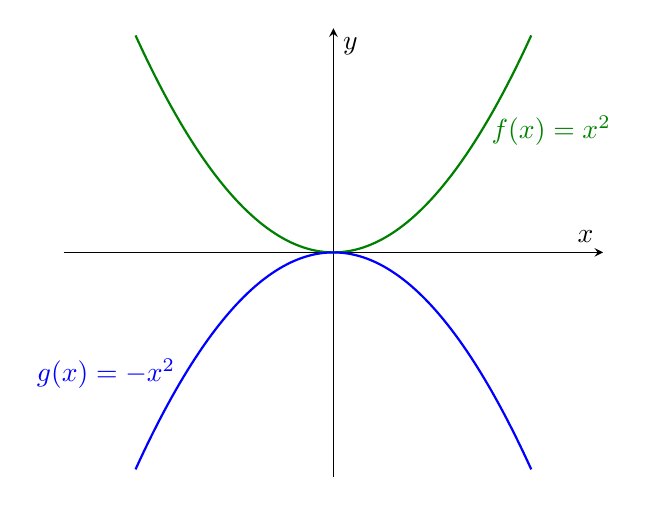
\begin{tikzpicture}[scale=1, every node/.style={scale=1}]
    \begin{axis}[
        axis lines=middle,
        xlabel=$x$, ylabel=$y$,
        xtick=\empty, ytick=\empty,
        xmin=-3, xmax=3,
        ymin=-5, ymax=5,
        samples=100,
        clip=false
    ]
    \addplot[domain=-2.2:2.2, green!50!black, thick, variable=\t] (\t, \t^2) node[right, pos=0.8] {$f(x) = x^2$};
    \addplot[domain=-2.2:2.2, blue, thick, variable=\t] (\t, -\t^2) node[left, pos=0.2] {$g(x) = -x^2$};
    \end{axis}
    \end{tikzpicture}
    \caption{Hàm $y=x^2$ (lồi) và $y=-x^2$ (lõm).}
    \label{fig:parabola-concavity}
\end{figure}
\end{example}

Nếu ta giả thiết thêm rằng $f''$ liên tục, thì tại điểm uốn $c$, $f''(c)$ phải bằng 0 (đây là hệ quả của Định lý giá trị trung gian áp dụng cho $f''$). Điều này cho phép ta tìm các \textit{ứng cử viên} cho điểm uốn bằng cách giải phương trình $f''(x)=0$, tương tự như cách ta tìm điểm dừng.

Tổng hợp lại, ta có thuật toán sau để phân tích hình dạng đồ thị.

\begin{importantbox}
\textbf{Xét tính lồi, lõm và tìm điểm uốn của hàm số:}
\begin{enumerate}[label={}]
    \item \textbf{Bước 1:} Tìm các điểm mà tại đó $f''(x)=0$ hoặc $f''(x)$ không xác định. Đây là các ứng cử viên cho điểm uốn.
    \item \textbf{Bước 2:} Lập bảng xét dấu cho $f''(x)$. Các điểm tìm được ở Bước 1 sẽ chia miền xác định thành các khoảng.
    \begin{itemize}
        \item Nếu $f''(x) > 0$ trên một khoảng, đồ thị \textbf{lồi} trên khoảng đó.
        \item Nếu $f''(x) < 0$ trên một khoảng, đồ thị \textbf{lõm} trên khoảng đó.
    \end{itemize}
    \item \textbf{Bước 3:} Nếu $f''(x)$ đổi dấu khi đi qua một điểm ứng cử viên $c$ (và $f$ liên tục tại $c$), thì $(c, f(c))$ là một \textbf{điểm uốn}.
\end{enumerate}
\end{importantbox}

\begin{example}
Xét tính lồi lõm và tìm điểm uốn của hàm số $f(x) = x^4 - 6x^2 -10$.

\textit{Lời giải.}
Ta đã tính được đạo hàm cấp hai của hàm số này trong ví dụ trước:
$$ f''(x) = 12x^2 - 12 = 12(x^2 - 1) $$
Giải phương trình $f''(x)=0$, ta được $x = \pm 1$. Đây là hai ứng cử viên cho điểm uốn. Ta lập bảng biến thiên cho $f''(x)$:

\begin{center}
\begin{tabular}{c|ccccccc}
$x$ & $-\infty$ & & $-1$ & & $1$ & & $+\infty$ \\
\hline
$f''(x)$ & & $+$ & $0$ & $-$ & $0$ & $+$ & \\
\hline
$f(x)$ & & lồi & điểm uốn & lõm & điểm uốn & lồi & \\
\end{tabular}
\end{center}
Từ bảng trên, ta kết luận:
\begin{itemize}
    \item Hàm số lồi trên các khoảng $(-\infty, -1)$ và $(1, +\infty)$.
    \item Hàm số lõm trên khoảng $(-1, 1)$.
    \item Hàm số có hai điểm uốn tại $x=-1$ (điểm $(-1, -1)$) và $x=1$ (điểm $(1, -1)$).
\end{itemize}
Kết quả này hoàn toàn khớp với đồ thị của hàm số đã được vẽ ở Hình \ref{fig:quartic-function-plot}. Từ đồ thị, ta khó có thể xác định chính xác tọa độ các điểm uốn nếu không có công cụ đạo hàm.
\end{example}

\subsubsection{Khảo sát và vẽ đồ thị của hàm số}
\label{subsubsec:graphing-functions}

Việc tổng hợp các thông tin về chiều biến thiên (từ đạo hàm cấp một) và tính lồi/lõm (từ đạo hàm cấp hai), kết hợp với việc tìm các điểm đặc biệt như giao điểm với các trục tọa độ và các tiệm cận (giới hạn ở vô cực hoặc tại các điểm gián đoạn), cho phép chúng ta phác họa được đồ thị của một hàm số một cách chi tiết và chính xác. Quy trình này đã được giới thiệu trong chương trình phổ thông và là một trong những ứng dụng tổng hợp quan trọng nhất của phép tính vi phân.

\begin{example}
Khảo sát và vẽ đồ thị hàm số $f(x) = x^3 - 3x^2 - 9x + 5$.

\textit{Lời giải.}
\textbf{1. Tập xác định:} $D = \R$.

\textbf{2. Đạo hàm cấp một và chiều biến thiên:}
$$ f'(x) = 3x^2 - 6x - 9 = 3(x^2 - 2x - 3) = 3(x+1)(x-3) $$
Phương trình $f'(x)=0$ có các nghiệm $x=-1$ và $x=3$. Đây là các điểm dừng của hàm số.

Ta lập bảng biến thiên cho $f'(x)$:

\begin{center}
  \begin{tikzpicture}
  % Khởi tạo bảng
  \tkzTabInit[lgt=2, espcl=2]%
    {$x$/1, $f'(x)$/1, $f(x)$/2}%
    {$-\infty$, $-1$, $3$, $+\infty$}

  % Dòng dấu của f'(x)
  \tkzTabLine{ , +, z, -, z, + }

  % Dòng biến thiên của f(x)
  \tkzTabVar{ -/ $-\infty$, +/ $10$, -/ $-22$, +/ $+\infty$ }

  % % Ghi chú Cực đại và Cực tiểu
  \node at (4.5,-2.8) {CT};
  \node at (6.55,-3.2) {CĐ};
  \end{tikzpicture}
\end{center}

Từ bảng trên, ta thấy:
\begin{itemize}
    \item Hàm số đồng biến trên các khoảng $(-\infty, -1)$ và $(3, +\infty)$.
    \item Hàm số nghịch biến trên khoảng $(-1, 3)$.
    \item Hàm số đạt cực đại tại $x=-1$, $f_{CD} = f(-1) = 10$.
    \item Hàm số đạt cực tiểu tại $x=3$, $f_{CT} = f(3) = -22$.
\end{itemize}

\textbf{3. Đạo hàm cấp hai và tính lồi/lõm:}
$$ f''(x) = 6x - 6 $$
Phương trình $f''(x) = 0$ có nghiệm $x=1$.

Bảng xét dấu cho $f''(x)$:
\begin{center}
\begin{tabular}{c|ccccc}
$x$ & $-\infty$ & & $1$ & & $+\infty$ \\
\hline
$f''(x)$ & & $-$ & $0$ & $+$ & \\
\hline
$f(x)$ & & lõm & điểm uốn & lồi & \\
\end{tabular}
\end{center}

Từ bảng trên, ta thấy: 
\begin{itemize}
    \item Đồ thị lõm trên khoảng $(-\infty, 1)$.
    \item Đồ thị lồi trên khoảng $(1, +\infty)$.
    \item Đồ thị có một điểm uốn tại $x=1$, là điểm $(1, -6)$.
\end{itemize}
\textbf{4. Đồ thị:}
Dựa trên các phân tích trên, ta có thể phác họa đồ thị của hàm số.

\begin{figure}[H]
    \centering
    \begin{tikzpicture}[scale=1, every node/.style={scale=0.8}]
    \begin{axis}[
        axis lines=middle, xlabel=$x$, ylabel=$y$,
        xmin=-4, xmax=6, ymin=-25, ymax=15,
        grid=major,
        samples=50
    ]
    \addplot[domain=-3.5:5, red!70!black, thick, variable=\t] (\t, {\t^3 - 3*\t^2 - 9*\t + 5});
    \node[pin 135: {$f(x) = x^3 - 3x^2 - 9x + 5$}] at (axis cs: 1,10) {};
    \end{axis}
    \end{tikzpicture}
    \caption{Đồ thị của hàm số $f(x) = x^3 - 3x^2 - 9x + 5$.}
    \label{fig:cubic-function-graph}
\end{figure}
\end{example}

Ngày nay, việc vẽ đồ thị của các hàm số sơ cấp trở nên dễ dàng nhờ vào các phần mềm máy tính chuyên dụng. Người học nên tận dụng các công cụ này để trực quan hóa các tính chất của hàm số và kiểm tra lại các kết quả tính toán của mình. Tuy nhiên, việc nắm vững các bước khảo sát thủ công là cực kỳ quan trọng để có thể hiểu sâu sắc mối liên hệ giữa hàm số, đạo hàm và hình dạng đồ thị của nó.

\begin{example}
Hình \ref{fig:geogebra-complex-plot} minh họa đồ thị của một hàm số phức tạp được vẽ bằng phần mềm GeoGebra. Mặc dù công thức hàm phức tạp, ta vẫn có thể nhận xét các tính chất của nó một cách trực quan từ đồ thị: hàm số có hai cực tiểu địa phương trong khoảng $(-1.5, -1)$ và $(-0.5, 0.5)$, một cực đại địa phương trong khoảng $(-1, -0.5)$ và hai điểm uốn, một gần $-1$ và một gần $-0.5$.

Bằng cách sử dụng các công cụ tính toán của phần mềm, ta có thể tìm được giá trị xấp xỉ của điểm các điểm cực tiểu là tại những điểm: $x \approx -1.23, x = 0$ , xấp xỉ của các cực đại là $x \approx 0.85$ và các điểm uốn tại $x \approx -1.1$ và $x \approx -0.55$.
\end{example}

% TODO: Người dùng tự chèn hình ảnh từ GeoGebra vào đây.
\begin{figure}[H]
    \centering
    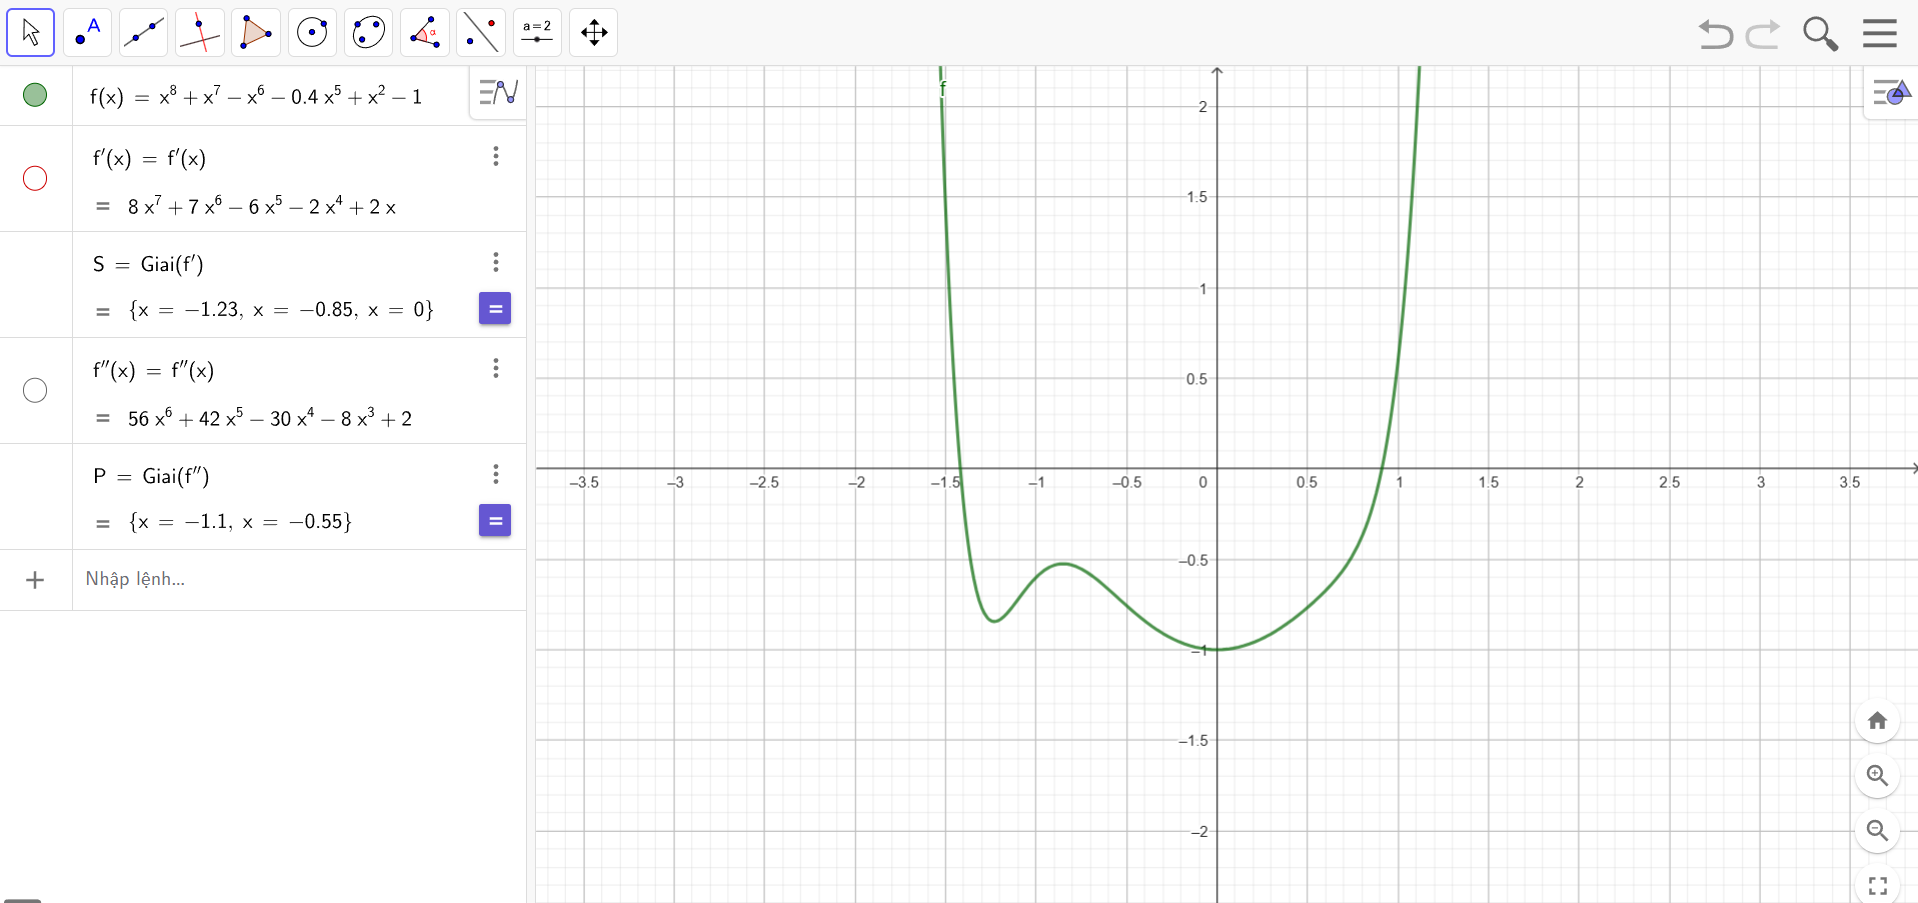
\includegraphics[width=1\textwidth]{figures/geogebra_Complex_Plot.png}
    \caption{Đồ thị hàm số phức tạp và các điểm đặc biệt.}
    \label{fig:geogebra-complex-plot}
\end{figure}

\subsubsection{Xấp xỉ tuyến tính}
\label{subsubsec:linear-approximation}

Từ định nghĩa đạo hàm tại một điểm $a$:
$$ f'(a) = \limit{x}{a} \dfrac{f(x) - f(a)}{x - a} $$
ta có thể thấy rằng khi $x$ ở rất gần $a$, tỉ số $\dfrac{f(x) - f(a)}{x - a}$ sẽ xấp xỉ bằng $f'(a)$. Điều này dẫn đến một trong những nguyên lý nền tảng và hữu dụng nhất của phép tính vi phân: \textbf{xấp xỉ tuyến tính}.

Nếu đặt $x = a+h$, khi $h \approx 0$, ta có:
$$ f'(a) \approx \dfrac{f(a+h) - f(a)}{h} \implies f(a+h) - f(a) \approx f'(a)h $$
Công thức này cho thấy sự thay đổi của hàm số, $\Delta y = f(a+h) - f(a)$, có thể được xấp xỉ bằng tốc độ thay đổi tức thời $f'(a)$ nhân với sự thay đổi nhỏ của biến số, $\Delta x = h$.

Về mặt hình học, nguyên lý này có ý nghĩa rất trực quan: tại một lân cận đủ nhỏ của điểm $(a, f(a))$, đồ thị của hàm số $y=f(x)$ được xấp xỉ rất tốt bởi đường tiếp tuyến của nó tại điểm đó. Phương trình của đường tiếp tuyến là $y = f(a) + f'(a)(x-a)$. Do đó, khi $x \approx a$:
$$ f(x) \approx f(a) + f'(a)(x-a) $$

\begin{figure}[H]
    \centering
    \begin{tikzpicture}[scale=0.9, every node/.style={scale=0.9}]
    \begin{axis}[
        axis lines=middle,
        xlabel=$x$, ylabel=$y$,
        xtick={1, 2.5}, ytick={1, 3.25},
        xticklabels={$a$, $x$},
        yticklabels={$f(a)$, $f(x)$},
        xmin=-0.5, xmax=4,
        ymin=-0.5, ymax=5,
        samples=100,
        clip=false
    ]
    % Đồ thị hàm số
    \addplot[domain=0:3.5, thick, blue!60] {0.5*x^2 + 0.5} node[pos=0.8, right] {$y=f(x)$};
    % Tiếp tuyến
    \addplot[domain=-0.2:3.5, thick, red!70] {1*(x-1) + 1} node[pos=0.9, right] {$y = f(a) + f'(a)(x-a)$};
    
    % Các điểm
    \addplot[only marks, mark=*] coordinates {(1,1)} node[above left] {$(a, f(a))$};
    \addplot[only marks, mark=*] coordinates {(2.5, 3.625)};

    % Đường dóng
    \draw[dashed] (axis cs:1,0) -- (axis cs:1,1);
    \draw[dashed] (axis cs:0,1) -- (axis cs:1,1);
    \draw[dashed] (axis cs:2.5,0) -- (axis cs:2.5, 3.625);
    \draw[dashed] (axis cs:0, 3.625) -- (axis cs:2.5, 3.625);
    
    \end{axis}
    \end{tikzpicture}
    \caption{\centering Ý nghĩa hình học của xấp xỉ tuyến tính: đồ thị hàm số (màu xanh) được xấp xỉ bởi đường tiếp tuyến (màu đỏ) tại lân cận điểm $a$.}
    \label{fig:linear-approximation}
\end{figure}

\begin{example}
Ước lượng giá trị của $\sqrt[3]{8.02}$.

\textit{Lời giải.}
Ta cần xấp xỉ giá trị của hàm $f(x) = \sqrt[3]{x}$ tại $x=8.02$. Ta chọn điểm $a=8$ vì ta dễ dàng tính được $f(8)=2$.
Đạo hàm của hàm số là $f'(x) = \dfrac{1}{3\sqrt[3]{x^2}}$.
Tại $a=8$, ta có $f'(8) = \dfrac{1}{3\sqrt[3]{8^2}} = \dfrac{1}{12}$.

Áp dụng công thức xấp xỉ tuyến tính:
$$ f(8.02) \approx f(8) + f'(8)(8.02 - 8) = 2 + \dfrac{1}{12}(0.02) = 2 + \dfrac{0.02}{12} \approx 2.001667 $$
Giá trị tính bằng máy tính là $2.001665...$, cho thấy phép xấp xỉ của chúng ta rất chính xác.
\end{example}

\begin{example}[Chi phí cận biên trong kinh tế]
Gọi $C(x)$ là tổng chi phí để sản xuất $x$ đơn vị sản phẩm. Khi quy mô sản xuất lớn, việc thay đổi sản lượng thêm 1 đơn vị có thể được xem là một thay đổi ``nhỏ''. Áp dụng nguyên lý xấp xỉ tuyến tính với $a=x$ và $h=1$, ta có:
$$ C(x+1) - C(x) \approx C'(x) \cdot 1 = C'(x) $$
Đại lượng $C(x+1) - C(x)$ chính là chi phí để sản xuất thêm đơn vị sản phẩm thứ $x+1$. Do đó, trong kinh tế học, đạo hàm $C'(x)$ được gọi là \textbf{chi phí cận biên} (marginal cost). Nó được dùng để ước tính chi phí phát sinh khi sản xuất thêm một đơn vị sản phẩm tại quy mô hiện tại.

Chẳng hạn, nếu $C'(1000) = 15$ (USD/sản phẩm), điều này có nghĩa là tại quy mô sản xuất 1000 sản phẩm, chi phí để sản xuất thêm sản phẩm thứ 1001 là xấp xỉ 15 USD.
\end{example}

\subsubsection{Phương pháp Newton giải gần đúng phương trình}
\label{subsubsec:newton-method}

Trong nhiều bài toán thực tế, việc tìm nghiệm chính xác của một phương trình $f(x)=0$ là rất khó hoặc không thể. Phương pháp Newton, được đặt theo tên của Isaac Newton, là một thuật toán lặp mạnh mẽ để tìm nghiệm xấp xỉ của phương trình.

Ý tưởng cốt lõi của phương pháp này là bắt đầu từ một giá trị dự đoán ban đầu $x_1$ gần với nghiệm thực. Sau đó, ta xấp xỉ hàm số $f(x)$ bằng đường tiếp tuyến của nó tại điểm $(x_1, f(x_1))$. Giao điểm của đường tiếp tuyến này với trục hoành sẽ cho ta một giá trị $x_2$, mà ta kỳ vọng là một xấp xỉ tốt hơn cho nghiệm so với $x_1$. Quá trình này được lặp lại để tạo ra một dãy các giá trị $x_1, x_2, x_3, \dots$ hội tụ nhanh chóng về nghiệm thực của phương trình.

Phương trình tiếp tuyến của đồ thị $y=f(x)$ tại điểm $(x_n, f(x_n))$ là:
$$ y - f(x_n) = f'(x_n)(x - x_n) $$
Để tìm giao điểm của tiếp tuyến với trục hoành, ta cho $y=0$ và giải phương trình tìm $x$. Giá trị $x$ này chính là $x_{n+1}$:
$$ 0 - f(x_n) = f'(x_n)(x_{n+1} - x_n) \implies x_{n+1} = x_n - \dfrac{f(x_n)}{f'(x_n)} $$
Đây chính là công thức lặp của phương pháp Newton.

% TODO: Hình này đang bị bug
% \begin{figure}[H]
%     \centering
%     \begin{tikzpicture}[scale=1, every node/.style={scale=1}]
%     \begin{axis}[
%         axis lines=middle, xlabel=$x$, ylabel=$y$,
%         xmin=-0.5, xmax=3, ymin=-2, ymax=4,
%         xtick=\empty, ytick=\empty,
%         samples=100
%     ]
%     % Đồ thị hàm số
%     \addplot[domain=0.5:2.8, thick, blue!70, name path=f] {x^3 - 3*x^2 + x + 2};
    
%     % Điểm ban đầu x1 và các điểm trên đồ thị
%     \node[below] at (axis cs:2.5, 0) {$x_1$};
%     \fill (axis cs:2.5, 0.875) circle (1.5pt);
    
%     % Tiếp tuyến tại x1
%     \addplot[domain=1.5:3, thick, red!70, name path=tan1] {4.75*(x-2.5) + 0.875};
    
%     % Giao điểm của tiếp tuyến và trục x -> x2
%     \path[name intersections={of=tan1 and axis, by={x2_point}}];
%     \node[below] at (x2_point) {$x_2$};
%     \fill (x2_point |- {axis cs:0, -0.63}) circle (1.5pt);
    
%     % Tiếp tuyến tại x2
%     \addplot[domain=1.5:2.5, thick, green!70!black, name path=tan2] {1.93*(x-2.315) - 0.63};
    
%     % Giao điểm của tiếp tuyến và trục x -> x3
%     \path[name intersections={of=tan2 and axis, by={x3_point}}];
%     \node[below] at (x3_point) {$x_3$};

%     % Giao điểm của đồ thị và trục x (nghiệm)
%     \path[name intersections={of=f and axis, by={root_point}}];
%     \node[below, xshift=2mm] at (root_point) {$r$};

%     % Đường dóng
%     \draw[dashed, gray] (axis cs:2.5, 0) -- (axis cs:2.5, 0.875);
%     \draw[dashed, gray] (x2_point) -- (x2_point |- {axis cs:0, -0.63});
    
%     \end{axis}
%     \end{tikzpicture}
%     \caption{Minh họa phương pháp Newton: bắt đầu từ $x_1$, ta tìm được $x_2$, rồi $x_3$ tiến dần về nghiệm thực $r$.}
%     \label{fig:newton-method}
% \end{figure}

\begin{example}
Sử dụng phương pháp Newton để tìm nghiệm xấp xỉ của phương trình $x^3 - x - 1 = 0$.

\textit{Lời giải.}
Đặt $f(x) = x^3 - x - 1$. Ta có $f'(x) = 3x^2 - 1$.
Công thức lặp của phương pháp Newton là:
$$ x_{n+1} = x_n - \dfrac{x_n^3 - x_n - 1}{3x_n^2 - 1} $$
Ta thấy $f(1) = -1$ và $f(2) = 5$, vậy phương trình có nghiệm trong khoảng $(1, 2)$. Ta chọn giá trị ban đầu là $x_1 = 1.5$.
\begin{align*}
    x_2 &= 1.5 - \dfrac{(1.5)^3 - 1.5 - 1}{3(1.5)^2 - 1} = 1.5 - \dfrac{0.875}{5.75} \approx 1.347826 \\
    x_3 &= 1.347826 - \dfrac{(1.347826)^3 - 1.347826 - 1}{3(1.347826)^2 - 1} \approx 1.325200 \\
    x_4 &= 1.325200 - \dfrac{(1.325200)^3 - 1.325200 - 1}{3(1.325200)^2 - 1} \approx 1.324718
\end{align*}
Chỉ sau vài bước lặp, ta đã thu được giá trị xấp xỉ của nghiệm với độ chính xác cao.
\end{example}

\subsubsection*{Phân tích sai số của xấp xỉ tuyến tính}
Ta có thể đánh giá độ chính xác của công thức xấp xỉ tuyến tính. Đặt phần dư (sai số) là:
$$ r(h) = f(a+h) - [f(a) + f'(a)h] $$
Khi đó, công thức xấp xỉ có thể được viết lại một cách chính xác là:
$$ f(a+h) = f(a) + f'(a)h + r(h) $$
Từ định nghĩa đạo hàm, ta có:
$$ \limit{h}{0} \dfrac{f(a+h) - f(a)}{h} - f'(a) = 0 $$
$$ \implies \limit{h}{0} \dfrac{f(a+h) - f(a) - f'(a)h}{h} = 0 \implies \limit{h}{0} \dfrac{r(h)}{h} = 0 $$
Điều này có nghĩa là sai số $r(h)$ tiến về $0$ nhanh hơn cả $h$. Trong giải tích, người ta gọi $r(h)$ là một \textit{vô cùng bé bậc cao hơn} so với $h$.

\subsection{Quy tắc L'Hôpital và ứng dụng trong tính giới hạn}
\label{sec:lhopital-rule}

Trong nhiều trường hợp, khi tính giới hạn của một thương $\dfrac{f(x)}{g(x)}$ lúc $x \to a$, ta gặp phải tình huống cả tử số $f(x)$ và mẫu số $g(x)$ cùng tiến về $0$ hoặc cùng tiến về $\infty$. Các trường hợp này được gọi là các \textbf{dạng vô định}, phổ biến nhất là $\dfrac{0}{0}$ và $\dfrac{\infty}{\infty}$. Khi đó, ta chưa thể kết luận ngay về giá trị của giới hạn.

Quy tắc L'Hôpital\footnote{Quy tắc được đặt theo tên của nhà toán học người Pháp Guillaume de l'Hôpital (thế kỷ 17), đọc là ``Lô-pi-tan''.} là một công cụ cực kỳ hiệu quả để giải quyết các dạng vô định này. Quy tắc phát biểu rằng, dưới một số điều kiện nhất định, giới hạn của thương hai hàm số bằng giới hạn của thương hai đạo hàm của chúng:
\begin{importantbox}
    \[\limit{x}{a} \dfrac{f(x)}{g(x)} = \limit{x}{a} \dfrac{f'(x)}{g'(x)}\]
\end{importantbox}

Ta có thể hiểu ý tưởng của quy tắc này thông qua xấp xỉ tuyến tính. Giả sử ta có dạng vô định $\dfrac{0}{0}$, với $f(a) = g(a) = 0$. Khi $x$ rất gần $a$, ta có:
$ f(x) \approx f(a) + f'(a)(x-a) = f'(a)(x-a) $
$ g(x) \approx g(a) + g'(a)(x-a) = g'(a)(x-a) $
Do đó, $ \dfrac{f(x)}{g(x)} \approx \dfrac{f'(a)(x-a)}{g'(a)(x-a)} = \dfrac{f'(a)}{g'(a)} $.
Để có một chứng minh chặt chẽ, ta sẽ sử dụng các Định lý giá trị trung bình.

\subsubsection*{Dạng vô định \texorpdfstring{$\dfrac{0}{0}$}{0/0}}

\begin{proposition}[Quy tắc L'Hôpital cho dạng 0/0]
\label{prop:lhopital-zero}
Giả sử $f$ và $g$ là các hàm khả vi trên một khoảng mở chứa $a$ (trừ khả năng tại $a$) và $g'(x) \neq 0$ trên khoảng đó (trừ khả năng tại $a$). Nếu
$$ \limit{x}{a} f(x) = 0 \quad \text{và} \quad \limit{x}{a} g(x) = 0 $$
và giới hạn $\limit{x}{a} \dfrac{f'(x)}{g'(x)}$ tồn tại (hữu hạn hoặc vô hạn), thì:
$$ \limit{x}{a} \dfrac{f(x)}{g(x)} = \limit{x}{a} \dfrac{f'(x)}{g'(x)} $$
Mệnh đề này vẫn đúng cho các giới hạn một phía ($x \to a^+$, $x \to a^-$) và giới hạn ở vô cùng ($x \to \infty$, $x \to -\infty$).
\end{proposition}

\begin{proof}
Ta chứng minh cho trường hợp $x \to a^+$. Các trường hợp khác có thể được suy ra một cách tương tự.
Định nghĩa hai hàm phụ $F$ và $G$ như sau:
$$ F(x) = \begin{cases} f(x) & \text{nếu } x > a \\ 0 & \text{nếu } x = a \end{cases} \quad \text{và} \quad G(x) = \begin{cases} g(x) & \text{nếu } x > a \\ 0 & \text{nếu } x = a \end{cases} $$
Do $\limit{x}{a^+} f(x) = 0$ và $\limit{x}{a^+} g(x) = 0$, các hàm $F$ và $G$ liên tục trên $[a, x)$ với mọi $x>a$. Áp dụng Định lý giá trị trung bình Cauchy (Định lý \ref{thm:cauchy-mean-value}) cho $F$ và $G$ trên đoạn $[a, x]$, tồn tại một số $c \in (a, x)$ sao cho:
$$ \dfrac{F(x) - F(a)}{G(x) - G(a)} = \dfrac{F'(c)}{G'(c)} $$
Thay định nghĩa của $F$ và $G$ vào, ta có:
$$ \dfrac{f(x) - 0}{g(x) - 0} = \dfrac{f'(c)}{g'(c)} \implies \dfrac{f(x)}{g(x)} = \dfrac{f'(c)}{g'(c)} $$
Khi cho $x \to a^+$, vì $a < c < x$ nên ta cũng có $c \to a^+$. Do đó:
$$ \limit{x}{a^+} \dfrac{f(x)}{g(x)} = \limit{c}{a^+} \dfrac{f'(c)}{g'(c)} $$
Điều này hoàn thành chứng minh.
\end{proof}

\begin{example}
Tính giới hạn $\limit{x}{1} \dfrac{x^3 - 1}{x^2 - 1}$.

\textit{Lời giải.}
Đây là dạng vô định $\dfrac{0}{0}$. Áp dụng quy tắc L'Hôpital:
$$ \limit{x}{1} \dfrac{x^3 - 1}{x^2 - 1} = \limit{x}{1} \dfrac{(x^3 - 1)'}{(x^2 - 1)'} = \limit{x}{1} \dfrac{3x^2}{2x} = \dfrac{3(1)^2}{2(1)} = \dfrac{3}{2} $$
\end{example}

\begin{example}
Tính giới hạn $\limit{x}{0} \dfrac{e^x - 1 - x}{x^2}$.

\textit{Lời giải.}
Đây là dạng vô định $\dfrac{0}{0}$.
$$ \limit{x}{0} \dfrac{e^x - 1 - x}{x^2} = \limit{x}{0} \dfrac{(e^x - 1 - x)'}{(x^2)'} = \limit{x}{0} \dfrac{e^x - 1}{2x} $$
Giới hạn mới vẫn là dạng vô định $\dfrac{0}{0}$. Ta tiếp tục áp dụng quy tắc L'Hôpital:
$$ \limit{x}{0} \dfrac{e^x - 1}{2x} = \limit{x}{0} \dfrac{(e^x - 1)'}{(2x)'} = \limit{x}{0} \dfrac{e^x}{2} = \dfrac{e^0}{2} = \dfrac{1}{2} $$
\end{example}

\subsubsection*{Dạng vô định \texorpdfstring{$\dfrac{\infty}{\infty}$}{\textinfty/\textinfty}}

\begin{proposition}[Quy tắc L'Hôpital cho dạng $\infty/\infty$]
\label{prop:lhopital-inf}
Giả sử $f$ và $g$ là các hàm khả vi trên khoảng $(a, b)$ và $g'(x) \neq 0$ với mọi $x \in (a, b)$. Nếu
$$ \limit{x}{a^+} f(x) = \pm\infty \quad \text{và} \quad \limit{x}{a^+} g(x) = \pm\infty $$
và giới hạn $\limit{x}{a^+} \dfrac{f'(x)}{g'(x)}$ tồn tại (là một số thực hoặc $\pm\infty$), thì:
$$ \limit{x}{a^+} \dfrac{f(x)}{g(x)} = \limit{x}{a^+} \dfrac{f'(x)}{g'(x)} $$
Mệnh đề vẫn đúng khi thay giới hạn $x \to a^+$ bằng các giới hạn $x \to b^-$, $x \to c$ với $c \in (a,b)$, hoặc khi $a = -\infty$ và $b = \infty$.
\end{proposition}

\begin{proof}
Ta chứng minh cho trường hợp $L = \limit{x}{a^+} \dfrac{f'(x)}{g'(x)}$ là một số thực hữu hạn.
Với một điểm $c \in (a,b)$ bất kỳ, ta có thể viết lại biểu thức như sau:
$$ \dfrac{f(x)}{g(x)} - L = \dfrac{f(c) - Lg(c)}{g(x)} + \left(1 - \dfrac{g(c)}{g(x)}\right) \left(\dfrac{f(x) - f(c)}{g(x) - g(c)} - L\right) $$
Cho trước một $\epsilon > 0$. Vì giới hạn của thương các đạo hàm tồn tại, ta có thể chọn $c$ đủ gần $a$ sao cho với mọi $x \in (a,c)$, ta có $\left|\dfrac{f'(x)}{g'(x)} - L\right| < \epsilon$.

Với mọi $x \in (a,c)$, áp dụng Định lý giá trị trung bình Cauchy cho đoạn $[x, c]$, tồn tại một số $\theta \in (x, c)$ sao cho:
$$ \dfrac{f(x) - f(c)}{g(x) - g(c)} = \dfrac{f'(\theta)}{g'(\theta)} $$
Do đó, $\left|\dfrac{f(x) - f(c)}{g(x) - g(c)} - L\right| = \left|\dfrac{f'(\theta)}{g'(\theta)} - L\right| < \epsilon$.

Mặt khác, vì $\limit{x}{a^+} g(x) = \pm\infty$, ta có thể chọn một điểm $c_1$ sao cho $a < c_1 < c$ và với mọi $x \in (a, c_1)$, các bất đẳng thức sau được thỏa mãn:
$$ \left|\dfrac{f(c) - Lg(c)}{g(x)}\right| < \epsilon \quad \text{và} \quad \left|1 - \dfrac{g(c)}{g(x)}\right| < 2 $$
Từ đó, với mọi $x \in (a, c_1)$, ta có:
$$ \left|\dfrac{f(x)}{g(x)} - L\right| < \epsilon + 2\epsilon = 3\epsilon $$
Vì $\epsilon$ có thể nhỏ tùy ý, điều này chứng tỏ $\limit{x}{a^+} \dfrac{f(x)}{g(x)} = L$. Các trường hợp khác được chứng minh tương tự như trong Mệnh đề \ref{prop:lhopital-zero}.
\end{proof}

\begin{example}
    Tính giới hạn $\limit{x}{\infty} \dfrac{5x + 3}{2x - 7}$.
    \begin{solution}
    Đây là dạng vô định $\dfrac{\infty}{\infty}$. Áp dụng quy tắc L'Hôpital:
    $$ \limit{x}{\infty} \dfrac{5x + 3}{2x - 7} \overset{L'H}{=} \limit{x}{\infty} \dfrac{(5x + 3)'}{(2x - 7)'} = \limit{x}{\infty} \dfrac{5}{2} = \dfrac{5}{2} $$
    \end{solution}
\end{example}

\begin{example}
Tính giới hạn $\limit{x}{\infty} \dfrac{\ln(x)}{\sqrt[3]{x}}$.
\begin{solution}
Đây là dạng vô định $\dfrac{\infty}{\infty}$.
$$ \limit{x}{\infty} \dfrac{\ln(x)}{\sqrt[3]{x}} \overset{L'H}{=} \limit{x}{\infty} \dfrac{(\ln x)'}{(x^{1/3})'} = \limit{x}{\infty} \dfrac{1/x}{\frac{1}{3}x^{-2/3}} = \limit{x}{\infty} \dfrac{3x^{2/3}}{x} = \limit{x}{\infty} \dfrac{3}{x^{1/3}} = 0 $$
\end{solution}
\end{example}

\begin{example}
    Chứng tỏ rằng hàm mũ $e^x$ tăng nhanh hơn bất kỳ hàm đa thức nào bằng cách tính $\limit{x}{\infty} \dfrac{x^3}{e^x}$.
    \begin{solution}
    Đây là dạng vô định $\dfrac{\infty}{\infty}$. Ta cần áp dụng quy tắc L'Hôpital nhiều lần.
    \begin{align*}
    \limit{x}{\infty} \dfrac{x^3}{e^x} &\overset{L'H}{=} \limit{x}{\infty} \dfrac{3x^2}{e^x} \quad \left(\text{vẫn là } \dfrac{\infty}{\infty}\right) \\
    &\overset{L'H}{=} \limit{x}{\infty} \dfrac{6x}{e^x} \quad \left(\text{vẫn là } \dfrac{\infty}{\infty}\right) \\
    &\overset{L'H}{=} \limit{x}{\infty} \dfrac{6}{e^x} = 0
    \end{align*}
    Kết quả này cho thấy khi $x$ tiến ra vô cùng, giá trị của $e^x$ tăng nhanh hơn rất nhiều so với $x^3$.
    \end{solution}
\end{example}

\subsubsection*{Các dạng vô định khác}

Quy tắc L'Hôpital cũng có thể được sử dụng để giải quyết các dạng vô định khác như $0 \cdot \infty$, $\infty - \infty$, $0^0$, $1^\infty$, và $\infty^0$. Phương pháp chung là tìm cách biến đổi các biểu thức này để đưa về dạng $\dfrac{0}{0}$ hoặc $\dfrac{\infty}{\infty}$.

\begin{example}[Dạng vô định $0 \cdot \infty$]
Tính giới hạn $\limit{x}{0^+} x \ln x$.
\begin{solution}
Giới hạn này có dạng $0 \cdot (-\infty)$. Ta có thể biến đổi nó thành dạng $\dfrac{\infty}{\infty}$ để áp dụng quy tắc L'Hôpital:
$$ \limit{x}{0^+} x \ln x = \limit{x}{0^+} \dfrac{\ln x}{1/x} $$
Bây giờ, ta có dạng $\dfrac{-\infty}{\infty}$. Áp dụng quy tắc L'Hôpital:
$$ \limit{x}{0^+} \dfrac{(\ln x)'}{(1/x)'} = \limit{x}{0^+} \dfrac{1/x}{-1/x^2} = \limit{x}{0^+} (-x) = 0 $$
\end{solution}
\end{example}

\begin{example}[Dạng vô định $\infty - \infty$]
Tính giới hạn $\limit{x}{1^+} \left(\dfrac{x}{x-1} - \dfrac{1}{\ln x}\right)$.
\begin{solution}
Đây là dạng vô định $\infty - \infty$. Ta quy đồng mẫu số để đưa về một phân thức duy nhất:
$$ \limit{x}{1^+} \dfrac{x \ln x - (x-1)}{(x-1)\ln x} $$
Khi $x \to 1^+$, cả tử và mẫu đều tiến về 0, tạo thành dạng vô định $\dfrac{0}{0}$. Áp dụng quy tắc L'Hôpital:
$$ \limit{x}{1^+} \dfrac{(x \ln x - x + 1)'}{((x-1)\ln x)'} = \limit{x}{1^+} \dfrac{\ln x + x\cdot\frac{1}{x} - 1}{\ln x + (x-1)\cdot\frac{1}{x}} = \limit{x}{1^+} \dfrac{\ln x}{\ln x + 1 - \frac{1}{x}} $$
Giới hạn này vẫn là dạng $\dfrac{0}{0}$. Ta áp dụng quy tắc L'Hôpital một lần nữa:
$$ \limit{x}{1^+} \dfrac{(\ln x)'}{(\ln x + 1 - \frac{1}{x})'} = \limit{x}{1^+} \dfrac{1/x}{1/x + 1/x^2} = \limit{x}{1^+} \dfrac{x}{x+1} = \dfrac{1}{2} $$
\end{solution}
\end{example}

Đối với các dạng vô định có dạng mũ, phương pháp phổ biến là lấy logarit tự nhiên của biểu thức.

\begin{example}[Dạng vô định $0^0$]
Tính giới hạn $\limit{x}{0^+} x^x$.
\begin{solution}
Đây là dạng vô định $0^0$. Đặt $y = x^x$, khi đó $\ln y = x \ln x$.
Ta đã tính ở ví dụ trước rằng $\limit{x}{0^+} x \ln x = 0$.
Vì hàm mũ là hàm liên tục, ta có:
$$ \limit{x}{0^+} x^x = \limit{x}{0^+} e^{\ln(x^x)} = e^{\limit{x}{0^+} (x \ln x)} = e^0 = 1 $$
\end{solution}
\end{example}

\begin{example}[Dạng vô định $1^\infty$ -- Ví dụ kinh điển]
Tính giới hạn $\limit{x}{\infty} \left(1 + \dfrac{1}{x}\right)^x$.
\begin{solution}
Đây là dạng vô định $1^\infty$. Đặt $y = \left(1 + \dfrac{1}{x}\right)^x$, suy ra $\ln y = x \ln\left(1 + \dfrac{1}{x}\right)$.
Giới hạn của $\ln y$ có dạng $\infty \cdot 0$. Ta biến đổi để có dạng $\dfrac{0}{0}$:
$$ \limit{x}{\infty} x \ln\left(1 + \dfrac{1}{x}\right) = \limit{x}{\infty} \dfrac{\ln(1 + 1/x)}{1/x} $$
Áp dụng quy tắc L'Hôpital:
$$ \limit{x}{\infty} \dfrac{\frac{-1/x^2}{1+1/x}}{-1/x^2} = \limit{x}{\infty} \dfrac{1}{1+1/x} = 1 $$
Do đó, $\limit{x}{\infty} \left(1 + \dfrac{1}{x}\right)^x = e^1 = e$.
Kết quả này rất quan trọng và thường được sử dụng:
\begin{importantbox}
$$ \limit{x}{\infty} \left(1 + \dfrac{1}{x}\right)^x = e $$
\end{importantbox}
\end{solution}
\end{example}

\begin{example}[Mô hình lãi nhập vốn liên tục]
Trong Ví dụ 1.2.6, ta đã khảo sát mô hình lãi nhập vốn sau những khoảng thời gian rời rạc và thu được công thức $A(t) = A(0)(1 + r)^t$. Mô hình này giả định rằng lãi chỉ được nhập vào vốn sau mỗi đơn vị thời gian (ví dụ: mỗi năm).

Tuy nhiên, trong thực tế, lãi có thể được nhập vốn thường xuyên hơn, chẳng hạn như hàng tháng, hàng ngày, hoặc thậm chí liên tục. Giả sử trong mỗi đơn vị thời gian (ví dụ: 1 năm), lãi được nhập vốn $n$ lần. Khi đó, lãi suất cho mỗi kỳ hạn là $\dfrac{r}{n}$, và sau $t$ đơn vị thời gian, số kỳ hạn sẽ là $nt$. Công thức tính lượng vốn tích lũy trở thành:
$$ A_n(t) = A(0)\left(1 + \dfrac{r}{n}\right)^{nt} $$
Mô hình \textbf{lãi nhập vốn liên tục} (hay còn gọi là lãi kép liên tục) là trường hợp giới hạn khi số lần nhập vốn trong một đơn vị thời gian, $n$, tiến ra vô cùng. Bài toán của chúng ta là tính giới hạn:
$$ A(t) = \limit{n}{\infty} A(0)\left(1 + \dfrac{r}{n}\right)^{nt} = A(0) \limit{n}{\infty} \left(1 + \dfrac{r}{n}\right)^{nt} $$
Để giải quyết giới hạn này, ta tập trung vào biểu thức $\limit{n}{\infty} \left(1 + \dfrac{r}{n}\right)^{nt}$. Ta nhận thấy nó có liên quan đến giới hạn kinh điển dùng để định nghĩa số $e$: $\limit{x}{\infty} \left(1 + \dfrac{1}{x}\right)^x = e$.

Ta thực hiện phép đổi biến. Đặt $x = \dfrac{n}{r}$. Khi $n \to \infty$, thì $x$ cũng tiến ra $\infty$. Từ đó, ta có $n = xr$. Thay vào biểu thức của giới hạn:
\begin{align*}
\limit{n}{\infty} \left(1 + \dfrac{r}{n}\right)^{nt} &= \limit{x}{\infty} \left(1 + \dfrac{r}{xr}\right)^{(xr)t} \\
&= \limit{x}{\infty} \left(1 + \dfrac{1}{x}\right)^{xrt} \\
&= \limit{x}{\infty} \left[ \left(1 + \dfrac{1}{x}\right)^x \right]^{rt}
\end{align*}
Vì hàm số $f(u) = u^{rt}$ là hàm liên tục, ta có thể đưa giới hạn vào bên trong:
$$ \left[ \limit{x}{\infty} \left(1 + \dfrac{1}{x}\right)^x \right]^{rt} = e^{rt} $$
Như vậy, ta thu được công thức cho mô hình tăng trưởng với lãi nhập vốn liên tục:
\begin{importantbox}
$$ A(t) = A(0)e^{rt} $$
\end{importantbox}
Công thức này không chỉ quan trọng trong lĩnh vực tài chính mà còn được ứng dụng rộng rãi để mô tả các quá trình tăng trưởng liên tục trong sinh học (tăng trưởng quần thể) và vật lý (phân rã phóng xạ).
\end{example}

\begin{example}[Dạng vô định $\infty^0$]
    Tính giới hạn $\limit{x}{\infty} (\ln x)^{1/x}$.
    \begin{solution}
    Đây là dạng vô định $\infty^0$. Đặt $y = (\ln x)^{1/x}$, suy ra $\ln y = \dfrac{\ln(\ln x)}{x}$.
    Giới hạn của $\ln y$ có dạng $\dfrac{\infty}{\infty}$. Áp dụng quy tắc L'Hôpital:
    $$ \limit{x}{\infty} \dfrac{\ln(\ln x)}{x} \overset{L'H}{=} \limit{x}{\infty} \dfrac{\frac{1/x}{ln(x)}}{1} = \limit{x}{\infty} \dfrac{1}{x \ln x} = 0 $$
    Vậy, $\limit{x}{\infty} (\ln x)^{1/x} = e^0 = 1$.
    \end{solution}
\end{example}

\subsection{Bài tập}

\subsubsection{Khảo sát và vẽ đồ thị hàm số}

% TAG: Phân tích đồ thị
\begin{exercise}
Từ đồ thị được cho ở Hình \ref{fig:ch4-ex-1}, hãy xác định và giải thích các tính chất sau của hàm số: miền xác định, các điểm gián đoạn, các điểm không khả vi, các khoảng tăng, giảm, các điểm cực trị địa phương và toàn cục, các khoảng lồi, lõm, và các điểm uốn.

% TODO: Người dùng chèn hình vẽ cho bài tập này.
% Đặt tên hình là fig:ch4-ex-1
\begin{figure}[H]
    \centering
    \begin{tikzpicture}
    \begin{axis}[
        width=0.9\textwidth,
        height=0.6\textwidth,
        xmin=-2, xmax=4.5,
        ymin=-1.5, ymax=4.5,
        axis lines=middle,
        xlabel=$x$,
        ylabel=$y$,
        xtick={-1, 1, 2, 3, 4},
        ytick={-1, 1, 2, 3, 4},
        grid=none,
        no marks,
        clip=false
    ]
    
    % Tiệm cận ngang y = 2
    \addplot[dashed, gray, domain=-2:4.5] {2};
    
    % Tiệm cận đứng x = 0.5
    \draw[dashed, gray] (axis cs:0.5,-1.5) -- (axis cs:0.5,4.5);
    
    % Nhánh trái (x < 0.5)
    \addplot[thick, smooth] coordinates {
        (-1.8,0.2) (-1.7,0.6) (-1.6,1.0) (-1.5,1.3)
        (-1.4,1.6) (-1.3,1.9) (-1.2,2.2) (-1.1,2.35)
        (-1.0,2.5) (-0.9,2.6) (-0.8,2.65) (-0.7,2.6)
        (-0.6,2.45) (-0.5,2.3) (-0.4,2.1) (-0.3,1.9)
        (-0.2,1.6) (-0.1,1.2) (0.0,0.9) (0.1,0.7)
        (0.2,0.6) (0.3,0.5) (0.4,0.45) (0.45, 0.42) (0.48, 0.405)
        (0.5, 0.4)
    };

    % Nhánh phải (x > 0.5)
    \addplot[thick, smooth] coordinates {
        (0.55, 4.2) (0.6,3.8) (0.7,3.2) (0.8,2.7) (0.9,2.3) 
        (1.0,2.0) (1.1,1.7) (1.2,1.4) (1.3,1.2) (1.4,1.05)
        (1.5,1.0) (1.6,1.05) (1.7,1.2) (1.8,1.5) (1.9,1.8)
        (2.0,2.1) (2.1,2.2) (2.2,2.15) (2.3,2.05) (2.4,1.9)
        (2.5,1.7) (2.6,1.55) (2.7,1.4) (2.8,1.25) (2.9,1.2)
        (3.0,1.25) (3.1,1.35) (3.2,1.45) (3.3,1.55) (3.4,1.65)
        (3.5,1.75) (3.6,1.85) (3.7,1.9) (3.8,1.95) (3.9,1.97)
        (4.0,1.975) (4.1,1.978) (4.2,1.98)
    };
    \end{axis}
    \end{tikzpicture}
    \caption{Hình minh họa cho bài tập}
    \label{fig:ch4-ex-1}
\end{figure}
\end{exercise}

\begin{exercise}
Yêu cầu tương tự với bài tập trên với Hình~\ref{fig:ch4-ex-2}
% TODO: Người dùng chèn hình vẽ cho bài tập này.
% Đặt tên hình là fig:ch4-ex-1
\begin{figure}[H]
    \centering
    \begin{tikzpicture}
    \begin{axis}[
        width=0.9\textwidth,
        height=0.6\textwidth,
        xmin=-2, xmax=4.5,
        ymin=-1.5, ymax=4.5,
        axis lines=middle,
        xlabel=$x$,
        ylabel=$y$,
        xtick={-1, 1, 2, 3, 4},
        ytick={-1, 1, 2, 3, 4},
        grid=none,
        no marks,
        clip=false
    ]
    
    % Tiệm cận ngang y = 2
    \addplot[dashed, gray, domain=-2:4.5] {2};
    
    % Vẽ đồ thị bằng cách nối các điểm
    \addplot[thick, smooth] coordinates {
        %--- PHẦN ĐÃ ĐƯỢC THAY THẾ (THEO HÌNH MÀU ĐỎ) ---
        (-1.5, 3.8) (-1.4, 3.68) (-1.3, 3.6) (-1.2, 3.5) (-0.8, 2.9) (-0.4, 2.4) 
        (0.0, 2.2) (0.4, 1.8) (0.8, 1.4) (1.2, 1.15) (1.3, 1.1)
        (1.3,1.1) (1.4,1.05)
        (1.5,1.0) (1.6,1.05) (1.7,1.2) (1.8,1.5) (1.9,1.8)
        (2.0,2.1) (2.1,2.2) (2.2,2.15) (2.3,2.05) (2.4,1.9)
        (2.5,1.7) (2.6,1.55) (2.7,1.4) (2.8,1.25) (2.9,1.2)
        (3.0,1.25) (3.1,1.35) (3.2,1.45) (3.3,1.55) (3.4,1.65)
        (3.5,1.75) (3.6,1.85) (3.7,1.9) (3.8,1.95) (3.9,1.97)
        (4.0,1.975) (4.1,1.978) (4.2,1.98)
    };
    \end{axis}
    \end{tikzpicture}
    \caption{Hình minh họa cho bài tập}
    \label{fig:ch4-ex-2}
\end{figure}
\end{exercise}

% TAG: Dữ liệu thực tế, Kinh tế
\begin{exercise}
% TODO: Cập nhật dữ liệu GDP mới nhất (ví dụ: 3 năm gần nhất)
Bảng dưới đây cung cấp dữ liệu về tốc độ tăng trưởng GDP của Việt Nam trong giai đoạn 2021-2023. Dựa vào các thông tin này, hãy phác họa một đồ thị có thể biểu diễn sự thay đổi của GDP theo thời gian, trong đó thể hiện rõ các nhận xét về tính tăng/giảm và lồi/lõm (tức là tốc độ tăng trưởng đang nhanh lên hay chậm lại).
\begin{center}
\begin{tabular}{|c|c|c|c|}
\hline
\textbf{Năm} & 2021 & 2022 & 2023 \\
\hline
\textbf{Tốc độ tăng trưởng GDP} & 2.58\% & 8.02\% & 5.05\% \\
\hline
\end{tabular}
\end{center}
\end{exercise}

% TAG: Diễn giải đồ thị, Kinh tế
\begin{exercise}
Mỗi đồ thị nhỏ dưới đây biểu diễn doanh thu của một công ty theo thời gian. Hãy nối mỗi phát biểu sau với đồ thị tương ứng và giải thích lựa chọn của bạn.
% TODO: Người dùng chèn 6 hình vẽ nhỏ cho bài tập này.

\begin{enumerate}[label=(\alph*)]
    \item Doanh thu đang tăng và tốc độ tăng trưởng ngày càng nhanh.
    \item Doanh thu đang giảm nhưng tốc độ giảm đang chậm lại.
    \item Doanh thu đang giảm và tình hình ngày càng tiêu cực hơn.
    \item Doanh thu vẫn tăng nhưng có dấu hiệu chững lại.
    \item Doanh thu đã từng giảm nhưng nay đang có dấu hiệu phục hồi.
    \item Doanh thu đã từng tăng trưởng tốt nhưng nay đang chậm dần.
\end{enumerate}
\end{exercise}

% TAG: Hàm cho bởi từng khoảng
\begin{exercise}
Cho hàm số $f(x) = \begin{cases} x^2+2x & \text{nếu } x \le 0 \\ \sin(x) & \text{nếu } 0 < x \le \pi \\ 1 & \text{nếu } x > \pi \end{cases}$.
\begin{enumerate}[label=(\alph*)]
    \item Tìm miền giá trị của $f$.
    \item Hàm $f$ liên tục trên những khoảng nào? Tìm các điểm gián đoạn.
    \item Tìm các điểm tới hạn của hàm số $f$.
    \item Vẽ đồ thị của hàm số $f$.
\end{enumerate}
\end{exercise}

% TAG: Diễn giải đồ thị, Kỹ năng tổng hợp
\begin{exercise}
Hãy phác họa đồ thị của một hàm số $f(x)$ thỏa mãn đồng thời tất cả các điều kiện sau:
\begin{enumerate}[label=(\alph*)]
    \item Cực đại địa phương tại $x=3$, giá trị $f(3) = 5$.
    \item Cực đại toàn cục tại $x=-2$, giá trị $f(-2) = 8$.
    \item Cực tiểu địa phương tại $x=1$, giá trị $f(1) = 0$.
    \item Các điểm uốn tại $x=-1$ và $x=2$.
    \item $\limit{x}{\infty} f(x) = -1$.
    \item $\limit{x}{-\infty} f(x) = -\infty$.
\end{enumerate}
\end{exercise}

% TAG: Kỹ năng tổng hợp, Vẽ đồ thị
\begin{exercise}
Phác họa đồ thị của một hàm số $f(x)$ liên tục trên $\R \setminus \{4\}$ và thỏa mãn đồng thời:
\begin{enumerate}[label=(\alph*)]
    \item $f'(x) > 0$ trên $(-\infty, -3)$ và $(1, 4)$.
    \item $f'(x) < 0$ trên $(-3, 1)$ và $(4, \infty)$.
    \item $f''(x) > 0$ trên $(-\infty, -1)$ và $(2, 4)$.
    \item $f''(x) < 0$ trên $(-1, 2)$.
    \item $\limit{x}{4} f(x) = \infty$.
    \item Hàm số có một tiệm cận ngang $y=1$.
\end{enumerate}
\end{exercise}

% TAG: Khảo sát hàm số, Cơ bản
\begin{exercise}
Với mỗi hàm số sau, hãy tìm các giá trị cực trị toàn cục, cực trị địa phương, các khoảng lồi, lõm, điểm uốn và phác họa đồ thị.
\begin{enumerate}[label=(\alph*)]
    \item $f(x) = x^3 - 6x^2 + 5$.
    \item $g(x) = \dfrac{x}{x^2+4}$.
    \item $h(x) = x\sqrt{5-x}$.
    \item $k(x) = x^2 e^{-x}$.
    \item $k(x) = x + \cos(2x)$ trên $[0, \pi]$.
\end{enumerate}
\end{exercise}

% TAG: Bài toán thêm, Tư duy phản biện
\begin{exercise}
Cho hàm số $f(x) = x^4 + ax^2 + b$.
\begin{enumerate}[label=(\alph*)]
    \item Tìm mối liên hệ giữa $a$ và $b$ để hàm số có đúng một điểm cực trị.
    \item Tìm mối liên hệ giữa $a$ và $b$ để hàm số có đúng ba điểm cực trị.
    \item Có thể tồn tại giá trị nào của $a$ và $b$ để hàm số có đúng hai điểm cực trị không? Giải thích.
\end{enumerate}
\end{exercise}

% TAG: Khoa học, Kinh điển, Mô hình hóa [Hàm số Sigmoid/Logistics cổ điển]
\begin{exercise}
Hàm số $f(x) = \dfrac{1}{1 + e^{-x}}$ được gọi là hàm \textit{sigmoid}\footnote{xem thêm tại \href{https://en.wikipedia.org/wiki/Sigmoid_function}{Wikipedia - Sigmoid Function}} hay một dạng đơn giản của hàm \textit{logistics}. Nó được sử dụng rất phổ biến trong các mô hình xác suất và mạng nơ-ron nhân tạo (machine learning).
\begin{enumerate}[label=(\alph*)]
    \item Khảo sát tính đơn điệu của hàm số.
    \item Khảo sát tính lồi, lõm và tìm điểm uốn của hàm số.
    \item Tìm các tiệm cận ngang và phác họa đồ thị của hàm số.
\end{enumerate}
\end{exercise}

% TAG: Khoa học, Kinh điển, Mô hình hóa [Hàm số Logistics tổng quát]
\begin{exercise}
Hàm số $f(x) = \dfrac{L}{1 + e^{-k(x-x_0)}}$ với $L, k, x_0$ là các hằng số dương, được gọi là hàm \textit{logistics} tổng quát\footnote{xem thêm tại \href{https://en.wikipedia.org/wiki/Logistic_function}{Wikipedia - Logistic Function}}. Nó xuất hiện thường xuyên trong các mô hình tăng trưởng bị giới hạn, chẳng hạn như sự lây lan của dịch bệnh hoặc tăng trưởng dân số trong một môi trường có nguồn tài nguyên hữu hạn.
\begin{enumerate}[label=(\alph*)]
    \item Khảo sát tính đơn điệu của hàm số. Tham số $k$ ảnh hưởng như thế nào đến tốc độ tăng trưởng?
    \item Chứng tỏ rằng hàm số có một điểm uốn tại $x = x_0$. Điểm này có ý nghĩa gì trong mô hình tăng trưởng? (Gợi ý: Đây là điểm mà tốc độ tăng trưởng đạt giá trị lớn nhất).
    \item Tìm các tiệm cận ngang của đồ thị. Tham số $L$ có ý nghĩa gì trong mô hình? Vẽ đồ thị của hàm.
\end{enumerate}
\end{exercise}

% TAG: Khoa học, Sinh học [Mô hình nồng độ thuốc]
\begin{exercise}
Nồng độ của một loại thuốc trong máu sau khi tiêm $t$ giờ được mô hình hóa bởi hàm $C(t) = \dfrac{At}{t^2 + B}$, trong đó $A$ và $B$ là các hằng số dương.
\begin{enumerate}[label=(\alph*)]
    \item Tìm thời điểm $t$ mà tại đó nồng độ thuốc trong máu là cao nhất.
    \item Tìm điểm uốn của đồ thị hàm số $C(t)$. Điểm uốn này có ý nghĩa thực tế là gì? (Gợi ý: Nó cho biết thời điểm mà tốc độ giảm nồng độ thuốc là nhanh nhất).
\end{enumerate}
\end{exercise}

% TAG: Kinh tế, Tối ưu hóa
\begin{exercise}
Một nhà sản xuất xác định rằng phương trình nhu cầu cho sản phẩm của họ là $p = 1200 - 3x$, trong đó $p$ là giá bán mỗi sản phẩm và $x$ là số sản phẩm bán được. Chi phí sản xuất $x$ sản phẩm là $C(x) = 5000 + 2x^2$.
\begin{enumerate}[label=(\alph*)]
    \item Viết hàm lợi nhuận $P(x)$.
    \item Cần sản xuất và bán bao nhiêu sản phẩm để đạt được lợi nhuận tối đa?
    \item Chứng tỏ rằng tại mức sản lượng cho lợi nhuận tối đa, doanh thu cận biên bằng chi phí cận biên.
\end{enumerate}
\end{exercise}

% TAG: Bài toán thêm, Vật lý, Kinh điển [Nguyên lý Fermat]
\begin{exercise}
Nguyên lý Fermat\footnote{xem thêm tại \href{https://en.wikipedia.org/wiki/Fermat's_principle}{Wikipedia - Fermat's principle}} trong quang học phát biểu rằng ánh sáng khi di chuyển từ điểm A đến điểm B sẽ đi theo con đường mất ít thời gian nhất. Giả sử ánh sáng di chuyển từ điểm $A(0, a)$ trong môi trường có vận tốc $v_1$ đến điểm $B(d, -b)$ trong môi trường có vận tốc $v_2$. Hai môi trường được ngăn cách bởi trục hoành $y=0$.
\begin{enumerate}[label=(\alph*)]
    \item Gọi $P(x, 0)$ là điểm mà tia sáng đi qua trên mặt phân cách. Hãy viết hàm số $T(x)$ biểu diễn tổng thời gian di chuyển của tia sáng từ A đến B.
    \item Bằng cách tìm giá trị nhỏ nhất của $T(x)$, hãy chứng minh rằng đường đi của tia sáng tuân theo \textbf{Định luật khúc xạ Snell}\footnote{xem thêm tại \href{https://en.wikipedia.org/wiki/Snell's_law}{Wikipedia - Snell's Law}}:
    $$ \dfrac{\sin \theta_1}{\sin \theta_2} = \dfrac{v_1}{v_2} $$
    trong đó $\theta_1$ và $\theta_2$ lần lượt là góc tới và góc khúc xạ.
\end{enumerate}
\end{exercise}

\subsubsection{Các bài toán tối ưu}

% TAG: Kinh tế, Tối ưu hóa
\begin{exercise}
Một cửa hàng bán các tác phẩm nghệ thuật. Họ ước tính rằng nếu bán 200 bản sao của một bức tranh, họ có thể định giá mỗi bản là 350 nghìn đồng. Tuy nhiên, để khuyến khích việc mua số lượng lớn, cứ mỗi bản bán thêm trên con số 200, họ sẽ giảm giá 10 nghìn đồng cho tất cả các bản đã bán thêm. Hỏi cửa hàng nên bán bao nhiêu bản sao để doanh thu đạt mức tối đa?
\end{exercise}

% TAG: Kinh tế, Kinh điển, Toàn diện [Phân tích Doanh thu, Chi phí và Lợi nhuận]
\begin{exercise}
Một công ty nghiên cứu thị trường và xác định rằng phương trình nhu cầu cho một sản phẩm của họ có thể được mô tả bởi $x = 180 - 15p$, trong đó $x$ là số đơn vị sản phẩm bán được trong một tháng và $p$ là giá của mỗi đơn vị sản phẩm (đơn vị: nghìn đồng).
\begin{enumerate}[label=(\alph*)]
    \item Tìm hàm doanh thu $R(x)$.
    \item Tìm hàm doanh thu cận biên (marginal revenue), $R'(x)$. Tính $R'(60)$ và giải thích ý nghĩa kinh tế của con số này.
    \item Giả sử hàm chi phí để sản xuất $x$ sản phẩm là $C(x) = 2x + 22.5$. Tìm hàm chi phí cận biên (marginal cost), $C'(x)$.
    \item Tìm hàm lợi nhuận $P(x)$.
    \item Tìm mức sản lượng $x$ để công ty đạt lợi nhuận tối đa.
    \item Tại mức sản lượng tối đa hóa lợi nhuận, hãy so sánh doanh thu cận biên và chi phí cận biên. Bạn có nhận xét gì?
    \item Tìm các điểm hòa vốn (break-even points), tức là các mức sản lượng mà tại đó lợi nhuận bằng không.
\end{enumerate}
\end{exercise}
 
% TAG: Kinh tế, Lý thuyết, Fact [Nguyên tắc Tối ưu hóa Lợi nhuận]
\begin{exercise}
Sử dụng các định nghĩa về hàm doanh thu $R(x)$, chi phí $C(x)$ và lợi nhuận $P(x) = R(x) - C(x)$, hãy chứng tỏ rằng nếu lợi nhuận đạt giá trị cực đại tại một mức sản lượng $x_0$ nào đó, thì tại điểm đó, doanh thu cận biên phải bằng chi phí cận biên, tức là $R'(x_0) = C'(x_0)$.
\end{exercise}
 
% TAG: Kinh tế, Lý thuyết, Fact [Chi phí Trung bình Cực tiểu]
\begin{exercise}
Gọi $C(x)$ là tổng chi phí để sản xuất $x$ đơn vị sản phẩm. Chi phí trung bình cho mỗi đơn vị sản phẩm được định nghĩa là $c(x) = \dfrac{C(x)}{x}$. Chứng tỏ rằng nếu hàm chi phí trung bình $c(x)$ đạt cực tiểu tại một mức sản lượng $x_0$, thì tại điểm đó, chi phí trung bình bằng với chi phí cận biên, tức là $c(x_0) = C'(x_0)$.
\end{exercise}

% TAG: Dữ liệu thực tế, Tối ưu hóa
\begin{exercise}
% _TODO_: Cập nhật dữ liệu mới nếu có
Dựa trên dữ liệu, tài sản của một quỹ đầu tư theo thời gian được mô hình hóa bởi hàm số:
$$ f(t) = -0.015t^4 + 0.35t^3 + 2.5t^2 + 60t + 500 \quad (0 \le t \le 40) $$
trong đó $f(t)$ là tài sản (tính bằng tỷ đồng) và $t$ là số năm kể từ năm 2000.
\begin{enumerate}[label=(\alph*)]
    \item Dùng phần mềm máy tính để vẽ đồ thị của hàm $f$.
    \item Vào năm nào thì tài sản của quỹ đạt mức cao nhất?
    \item Dựa vào mô hình, khi nào thì tài sản của quỹ bắt đầu giảm?
    \item Trong kinh tế, ta có trường hợp Quỹ có thể bị vỡ (tải sản còn lại bằng 0) nếu như số người đóng bảo hiểm không tằng lên hoặc quyền lợi của người mua bảo hiểm không bị giảm xuống. Dựa vào mô hình này, hãy cho biết khi nào thì Quỹ sẽ bị vỡ?
\end{enumerate}
\end{exercise}

% TAG: Khoa học, Nông nghiệp, Mô hình hóa
\begin{exercise}
Một mô hình được sử dụng để ước tính năng suất $Y$ của một loại cây trồng dựa trên nồng độ nitơ $N$ trong đất là:
$$ Y(N) = \dfrac{k \cdot N}{1 + N^2} $$
với $k$ là một hằng số dương phụ thuộc vào loại cây trồng. Tìm nồng độ nitơ trong đất để năng suất cây trồng đạt mức tối đa.
\end{exercise}

% TAG: Khoa học, Dịch tễ học
\begin{exercise}
Trong một quần thể động vật, tỷ lệ phần trăm bị nhiễm một loại bệnh sau $t$ ngày được mô hình hóa bởi hàm $p(t) = 10te^{-t/8}$. Hỏi sau bao nhiêu ngày thì tỷ lệ động vật bị nhiễm bệnh là lớn nhất?
\end{exercise}

% TAG: Khoa học, Sinh học
\begin{exercise}
Một hồ nước bị ô nhiễm vi khuẩn và được xử lý bằng hóa chất. Sau $t$ ngày, số lượng vi khuẩn trên mỗi mililit nước được cho bởi hàm:
$$ N(t) = 40 \left( \dfrac{t}{12} - \ln\left(\dfrac{t}{12}\right) \right) \quad \text{với } 1 \le t \le 20 $$
Tìm số lượng vi khuẩn ít nhất và nhiều nhất trong khoảng thời gian này và cho biết chúng xảy ra vào thời điểm nào.
\end{exercise}

% TAG: Vật lý, Kinh điển
\begin{exercise}
Một viên đạn được bắn lên với vận tốc đầu $v_0$ và góc bắn $\alpha$ so với phương ngang. Bỏ qua sức cản của không khí, tầm bay xa của viên đạn được cho bởi công thức $R(\alpha) = \dfrac{v_0^2 \sin(2\alpha)}{g}$, trong đó $g$ là gia tốc trọng trường. Tìm góc bắn $\alpha$ để viên đạn bay xa nhất.
\end{exercise}

% TAG: Tối ưu hóa, Hình học
\begin{exercise}
Trong tất cả các hình tam giác cân có cùng chu vi là $P$, hãy tìm tam giác có diện tích lớn nhất.
\end{exercise}

% TAG: Tối ưu hóa, Hình học, Kinh điển
\begin{exercise}
Một lon nước ngọt hình trụ có dung tích 330 ml (330 cm$^3$). Hãy tìm kích thước của lon (bán kính và chiều cao) để lượng vật liệu làm lon (diện tích bề mặt) là nhỏ nhất.
\end{exercise}

% TAG: Tối ưu hóa, Hình học
\begin{exercise}
Một hộp kim loại không nắp có đáy hình vuông. Tìm kích thước của hộp để thể tích đạt 2000 cm$^3$ và lượng kim loại sử dụng là ít nhất.
\end{exercise}

\subsubsection{Xấp xỉ tuyến tính và Phương pháp Newton}

% TAG: Tính toán, Xấp xỉ tuyến tính
\begin{exercise}
Sử dụng xấp xỉ tuyến tính tại một điểm thích hợp để ước lượng các giá trị sau:
\begin{enumerate}[label=(\alph*)]
    \item $(2.99)^3$
    \item $\cos(29^\circ)$
    \item $\sqrt[3]{26}$
    \item $\dfrac{1}{1.998}$
    \item $\tan(46^\circ)$
    \item $\sqrt{80.5}$
\end{enumerate}
\end{exercise}

% TAG: Kinh điển, Lý thuyết
\begin{exercise}
Bằng cách sử dụng xấp xỉ tuyến tính tại $x=0$, hãy kiểm tra các công thức xấp xỉ sau, vốn rất hữu ích trong khoa học và kỹ thuật khi $x$ có giá trị đủ nhỏ:
\begin{enumerate}[label=(\alph*)]
    \item $\sin x \approx x$
    \item $e^x \approx 1 + x$
    \item $\ln(1+x) \approx x$
\end{enumerate}
\end{exercise}

% TAG: Tính toán, Ứng dụng xấp xỉ
\begin{exercise}
Cho hàm số $f(x) = \ln(1 + x)$.
\begin{enumerate}[label=(\alph*)]
    \item Tìm xấp xỉ tuyến tính của hàm số $f(x)$ tại $x=0$.
    \item Áp dụng kết quả trên để xấp xỉ các giá trị $\ln(1.05)$ và $\ln(0.98)$.
\end{enumerate}
\end{exercise}

% TAG: Tính toán, Ứng dụng xấp xỉ
\begin{exercise}
Cho hàm số $f(x) = \sqrt[4]{15 + x^2}$.
\begin{enumerate}[label=(\alph*)]
    \item Tìm xấp xỉ tuyến tính của hàm số $f(x)$ tại $x=1$.
    \item Áp dụng kết quả trên để ước lượng giá trị của $\sqrt[4]{15.21}$ và $\sqrt[4]{14.84}$.
\end{enumerate}
\end{exercise}

% TAG: Kinh điển, Lý thuyết, Fact
\begin{exercise}
Chứng minh công thức xấp xỉ nhị thức tổng quát: với $k \in \R$ và $x \approx 0$, ta có:
$$ (1+x)^k \approx 1 + kx $$
Từ đó, hãy suy ra các công thức xấp xỉ thường gặp sau khi $|x|$ rất nhỏ:
\begin{enumerate}[label=(\alph*)]
    \item $\sqrt{1+x} \approx 1 + \dfrac{x}{2}$
    \item $\dfrac{1}{1-x} \approx 1 + x$
\end{enumerate}
\end{exercise}

% TAG: Ứng dụng, Vật lý
\begin{exercise}
Một vỏ cầu bằng kim loại có đường kính ngoài là 2 m và độ dày của vỏ là 0.5 mm. Hãy dùng xấp xỉ tuyến tính (hay vi phân) để ước tính thể tích của lượng kim loại đã được sử dụng để làm vỏ cầu. (Gợi ý: Thể tích hình cầu có bán kính $R$ là $V = \dfrac{4}{3}\pi R^3$).
\end{exercise}

% TAG: Phương pháp số
\begin{exercise}
Sử dụng phương pháp Newton để tính giá trị của $\sqrt{5}$ với giá trị ban đầu là $x_1 = 2$. Hãy thực hiện 3 bước lặp và so sánh kết quả với giá trị tính bằng máy tính.
\end{exercise}

% TAG: Phương pháp số
\begin{exercise}
Sử dụng phương pháp Newton để tìm một nghiệm xấp xỉ của phương trình $x^3 + 2x - 2 = 0$ với độ chính xác đến 4 chữ số thập phân. (Gợi ý: Bắt đầu với $x_1 = 1$).
\end{exercise}

\subsubsection{Quy tắc L'Hôpital}

% TAG: Luyện tập, Cấp độ Dễ
\begin{exercise}[Quy tắc L'Hôpital - Cấp độ Cơ bản]
Tính các giới hạn sau sử dụng Quy tắc L'Hôpital:
\begin{enumerate}[label=(\alph*)]
    \item $\limit{x}{2} \dfrac{x^2 - 4}{x - 2}$
    \item $\limit{x}{0} \dfrac{e^{3x} - 1}{x}$
    \item $\limit{x}{\infty} \dfrac{\ln x}{x}$
    \item $\limit{x}{0} \dfrac{\sin(5x)}{x}$
\end{enumerate}
\end{exercise}

% TAG: Luyện tập, Cấp độ Trung bình
\begin{exercise}[Quy tắc L'Hôpital - Cấp độ Trung bình]
Tính các giới hạn sau. Có thể cần áp dụng quy tắc nhiều lần hoặc biến đổi về dạng thích hợp.
\begin{enumerate}[label=(\alph*)]
    \item $\limit{x}{0^+} (\sin x)(\ln x)$
    \item $\limit{x}{\infty} x^2 e^{-x}$
    \item $\limit{x}{1^+} \left( \dfrac{x}{x-1} - \dfrac{1}{\ln x} \right)$
    \item $\limit{x}{(\pi/2)^-} (\tan x)^{\cos x}$
\end{enumerate}
\end{exercise}

% TAG: Luyện tập, Cấp độ Khó
\begin{exercise}[Quy tắc L'Hôpital - Cấp độ Nâng cao]
Tính các giới hạn sau:
\begin{enumerate}[label=(\alph*)]
    \item $\limit{x}{1} \dfrac{x^x - x}{\ln x - x + 1}$
    \item $\limit{x}{0} \dfrac{\cos(2x) - 1 + 2x^2}{x^4}$
    \item $\limit{x}{0^+} (\sin x)^{\tan x}$
    \item $\limit{x}{\infty} \left(x - \sqrt{x^2 + x}\right)$
\end{enumerate}
\end{exercise}

% TAG: Lý thuyết, Phản ví dụ
\begin{exercise}
Hãy xem xét giới hạn sau: $\limit{x}{\infty} \dfrac{x - \sin x}{x + \sin x}$.
\begin{enumerate}[label=(\alph*)]
    \item Chứng tỏ rằng đây là dạng vô định $\dfrac{\infty}{\infty}$.
    \item Nếu áp dụng Quy tắc L'Hôpital một cách máy móc, ta sẽ nhận được kết quả gì? Giới hạn của thương các đạo hàm có tồn tại không?
    \item Hãy tính giới hạn này bằng một phương pháp khác (ví dụ: chia cả tử và mẫu cho $x$).
    \item Bài toán này cho ta lưu ý gì về điều kiện áp dụng của Quy tắc L'Hôpital?
\end{enumerate}
\end{exercise}

\subsubsection{Các bài toán khác}

% TAG: Kinh điển, Fact, So sánh tốc độ tăng
\begin{exercise}
Chứng tỏ rằng với mọi số nguyên dương $n$, ta có:
$$ \limit{x}{\infty} \dfrac{x^n}{e^x} = 0 $$
Kết quả này thể hiện rằng hàm mũ $e^x$ tăng nhanh hơn bất kỳ hàm đa thức nào khi $x \to \infty$.
\end{exercise}

% TAG: Kinh điển, Fact, So sánh tốc độ tăng
\begin{exercise}
Chứng tỏ rằng với mọi số thực dương $\alpha$, ta có:
$$ \limit{x}{\infty} \dfrac{\ln x}{x^\alpha} = 0 $$
Điều này có ý nghĩa gì về tốc độ tăng của hàm logarit so với hàm lũy thừa?
\end{exercise}

% TAG: Khảo sát hàm, Kinh điển
\begin{exercise}
Cho hàm số $f(x) = x^{1/x}$ với $x > 0$.
\begin{enumerate}[label=(\alph*)]
    \item Tính $\limit{x}{\infty} f(x)$.
    \item Tìm $f'(x)$ và khảo sát chiều biến thiên của hàm số.
    \item Dựa vào kết quả trên, hãy so sánh hai số $e^{1/e}$ và $\pi^{1/\pi}$ mà không dùng máy tính.
\end{enumerate}
\end{exercise}

% TAG: Bất đẳng thức, Quy nạp
\begin{exercise}
Sử dụng phương pháp quy nạp toán học và kiến thức về đạo hàm để chứng minh bất đẳng thức sau đúng với mọi số nguyên dương $n$ và mọi $x \ge 0$\footnote{xem thêm tại \href{https://en.wikipedia.org/wiki/Taylor_series}{Khai triển Taylor}}:
$$ e^x \ge 1 + x + \dfrac{x^2}{2!} + \dots + \dfrac{x^n}{n!} $$
\end{exercise}

% TAG: Lý thuyết, Mở rộng
\begin{exercise}
Xét hàm số $f(x) = x^4$.
\begin{enumerate}[label=(\alph*)]
    \item Chứng tỏ rằng tại $x=0$, cả tiêu chuẩn đạo hàm bậc nhất và bậc hai đều không đưa ra kết luận về cực trị.
    \item Hãy sử dụng đạo hàm cấp cao hơn (cụ thể là đạo hàm cấp 4) để chứng tỏ rằng $f(x)$ đạt cực tiểu địa phương tại $x=0$.
    \item Từ đó, hãy phát biểu một tiêu chuẩn tổng quát sử dụng đạo hàm cấp $n$ để xác định cực trị trong trường hợp các đạo hàm cấp thấp hơn bằng không.
\end{enumerate}
\end{exercise}
